\documentclass[a4paper,12pt]{article}

\usepackage{titlesec} %za renewcommand
\usepackage{titling} %za renewcommand
\usepackage{ragged2e} %za na pr. flushleft
\usepackage{fancyhdr}
\usepackage{enumitem}
\usepackage{pdflscape}
\usepackage{array}
%\usepackage{tabularx}
\usepackage{makecell} %multiline cells + other non multiline cell are centered horiz. and vert.
\usepackage[table]{xcolor}
\usepackage{geometry}
\usepackage{hyperref}
\usepackage{booktabs}
\usepackage{color, soul}
\usepackage{gensymb}
\usepackage{graphicx}
\usepackage{verbatim} %comment sections
\usepackage{makecell}


\usepackage{array}                                                                                                                                               
\newcolumntype{L}[1]{>{\raggedright\let\newline\\\arraybackslash\hspace{0pt}}m{#1}}
\newcolumntype{C}[1]{>{\centering\let\newline\\\arraybackslash\hspace{0pt}}m{#1}}
\newcolumntype{R}[1]{>{\raggedleft\let\newline\\\arraybackslash\hspace{0pt}}m{#1}}

\geometry{left=1.5cm,right=1.5cm,top=2cm,bottom=2cm}

\setcounter{page}{0}
\setcounter{section}{-1}
\setcounter{secnumdepth}{4}

\titleformat{\paragraph}
{\normalfont\normalsize\bfseries}{\theparagraph}{1em}{}
\titlespacing*{\paragraph}
{0pt}{3.25ex plus 1ex minus .2ex}{1.5ex plus .2ex}

\pagestyle{fancy}
\fancyhf{}
\lfoot{Powerd by \LaTeX}
\cfoot{Verzija 1.7}
\rfoot{Stran: \thepage}

\newcommand{\mlc}[1]{\raisebox{0ex}{\makecell{#1}}}

\renewcommand{\headrulewidth}{0.5pt}
\renewcommand{\footrulewidth}{0.5pt}

\renewcommand{\maketitle}{
	\begin{center}
	{\huge\bfseries
	\thetitle}
	\end{center}

	\vspace{1cm}

	\centerline{\textbf{Naročnik: Šaj d.o.o.}}
	\centerline{\textbf{Vodja projekta: Anton Zhezhov}}

	\vspace{1cm}

	\leftline{\textbf{Začetek: 09.10.2019 } \hfill \textbf{Konec: 07.02.2020}}

	\vspace{4cm}

	\begin{center}
	
			\begin{tabular}{c|c|c|c}
					Ime in Priimek&Vloga	  &e - Naslov						&Opomba\\
				\hline
					Anton Zhezhov &Preverjanje&anton.zhezhov@student.um.si & 		\\
				\hline
					Žiga Zorc	  &Razvoj	  &ziga.zorc@student.um.si 	   &		\\
			\end{tabular}
	
	\end{center}
}

\let\oldtitleline\titleline
\renewcommand{\titleline}{\oldtitleline*}

\title{Projekt CSUPP}
\author{Anton Zhezhov}


\begin{document}

%underline color options for "paramteri"
\setul{0.6ex}{0.17ex}
\definecolor{Red}{rgb}{1,0.0,0.6}
\setulcolor{Red}



\maketitle

\setlength{\titlewidth}{16cm}

\newpage

\section{Naročnikove zahteve}
	\subsection{Splošne informacije}
			\begin{center}
				\begin{tabular}{c|c}
						Dokument & Verzija 1.0 \\
						\hline
						Naročnik & Šaj d.o.o. \\
						\hline
						Lokacija dokumenta & \href{https://github.com/antonzezov/OPI\_LV\_csupp/tree/master/doc01}{Github url} \\ %za zdaj ni public
						\hline
						Odgovorna oseba & Direktor podetja Šaj d.o.o. \\
				\end{tabular}
			\end{center}
	\subsection{Zahteve}
 
	\hspace{1em} V podjetju Šaj d.o.o. se ukvarjamo z razvojem inovativnih rešitev na področju 
	avtomatizacije in digitalizacije upravljanja poslovnih prostorov. Pri načrtovanju 
	naših rešitev dajemo velik poudarek na okoljsko trajnost, energetsko učinkovitost 
	ter ergonomičnost produktov, saj se zavedamo, da omenjene lastnosti pozitivno vplivajo 
	tako na izboljšano uporabniško izkušnjo kot na optimizacijo poslovanja skozi nižanje 
	stroškov.
	
	V podjetju smo prepoznali pomanjkanje rešitev, ki bi celovito naslovile 
	problem zastarelosti poslovnih prostorov. V ta namen načrtujemo razvoj centralnega 
	sistema za upravljanje poslovnega prostora, s čimer se nadejamo preboja na trg 
	in s tem izboljšanja poslovnega uspeha. Projekt že ima izoblikovano idejno zasnovo, 
	in sicer tako glede strojne opreme kot izgleda in funkcionalnosti. Sedaj smo v fazi 
	iskanja resnega partnerja, ki bi prevzel razvoj programske opreme. Ker želimo preveriti 
	osnovni koncept in delovanje centralnega sistema za upravljanje prostora, naj bo program 
	napisan v obliki simulatorja. Najprej potrebujemo preprost simulator brez grafičnega 
	vmesnika, ki bo izdelan kot konzolna aplikacija v jeziku C++ v integriranem razvojnem 
	okolju Visual Studio. Od simulatorja pričakujemo brezhibno in robustno delovanje v 
	operacijskem sistemu Windows. Poleg tega mora biti simulator hiter in preprost za uporabo. 
	Simulator naj omogoča krmiljenje temperature, vlage in osvetljenosti prostora. Predpogoj 
	je, da uporabnik v tekstovno datoteko vpiše želene ambientalne lastnosti v obliki: 
	
	TEMPERATURA: vrednost 

	VLAZNOST: vrednost v obliki relativne vlažnosti [\%] 

	OSVETLJENOST: vrednost v luksih [lx] 
	\\
	V datoteki naj bo še: 

	INTERVAL TEMPERATURE: [10,40]
	
	STOPNJA VLAZNOSTI: [30,60]

	INTERVAL OSVETLJENOSTI: [10,10000] 
	\\
	Simulator naj pred pričetkom prebere 
	vrednosti iz datoteke, nato pa naj omogoča izbiro med tremi načini delovanja: 

	1. Testni način: Uporabnik v program vnese dejansko temperaturo v prostoru. Računalnik vneseno 
	temperaturo pretvori v ostale relevantne merske enote. Nato naj izračuna razliko do 
	želene temperature (v vseh izbranih merskih enotah) in izvede ukaz za regulacijo 
	temperature. Analogno naj simulator omogoča vpis, izračun in izvedbo ukazov še za 
	vlažnost in osvetljenost. Simulacija se izvaja, dokler je ne prekine uporabnik. 
	
	2. Avtomatski način: Računalnik naj si izmisli dejansko temperaturo na intervalu 
	podanem v datoteki, pri čemer jo pretvori v najpomembnejše preostale merske enote. 
	Izmisli naj si še relativno stopnjo vlažnosti, in sicer med 30 in 60 \%, ter osvetljenost 
	na intervalu z datoteke. Nato naj za vsako posamezno meritev izračuna odstopanje od 
	želenih vrednosti ter izvede ukaze za popravek. Simulator naj izvede 100 meritev, pri 
	čemer izvede posamezno meritev vsake 3 sekunde. Na koncu simulacije naj izračuna 
	povprečno vrednost meritev ter povprečno odstopanje od želenih vrednosti za posamezne 
	\hyperlink{subsection.1.8}{\ul{parametre}}. 

	3. Avtomatski način 2: Simulator naredi isto kot v točki 2, pri čemer 
	naj uporabniku omogoča izbiro pri številu meritev in časovnem razmiku med njimi. 
	Izvajalec mora natančno slediti vsem internim standardom in poskrbeti za dokumentacijo. 
	
	Sestavni del projekta sta tudi razvijalska dokumentacija in uporabniški priročnik. 
	Od izvajalca pričakujemo, da do 24. 10. 2019 do 23.55 odda plan projekta, ki vključuje ceno. 
	Program in dokumentacija morata biti oddana najkasneje 23. 1. 2020 do 23.55. 
	Projekt bo plačan po posameznih zaključenih fazah. Za vsak teden zamude bo odbitih 10 \% plačila. 
	\\
	
	\leftline{Maribor 01.10.2019} 

	\hfill Direktor podjetja Šaj d.o.o.	

\newpage

\section{Plan projekta}

	\subsection{Kratek opis problema}

		\hspace{1em} Podjetje Šaj d.o.o. (v nadaljevanju naročnik) je dne 1. 10. 2019 naročilo 
		razvoj centralnega sistema za upravljanje poslovnega prostora.
		
		Naročnik želi optimizirati svoje poslovne prostore z avtomatiziranim sistemom, 
		ki meri in upravlja s paramteri. Sistem je preprost "simulator", ki je sposoben 
		prilagajanja \hyperlink{subsection.1.8}{\ul{parametrov}} tako avtomatsko kot na specifične uporabnikove zahteve.
		\subsubsection{Globalni cilji(globalne zahteve), ki jih želimo s produktom doseči}

		\begin{itemize}
				\item Izdelati simulator, ki primerno regulira {\hyperlink{subsection.1.8}{\ul{parametre}}} v prostoru
			\item Simulator mora biti hiter in preprost za uporabo
		\end{itemize}

		\subsubsection{Omejitve}

				\begin{itemize}
					\item Programski jezik: C++
					\item Operacijski sistem: Windows
					\item Izdelan mora biti kot simulator
					\item Konzolna aplikacija oz. brez grafičnega vmesnika
				\end{itemize}

		\subsubsection{Rok za zaključitev projekta, skupni stroški}

				\begin{itemize}
					\item Do 22.10.2019 do 23:55 oddan plan projekta 
					\item Do 23.01.2020 do 23:55 oddan projekt
				\end{itemize}

		\subsubsection{Funkcije}

				\begin{itemize}
						\item Pretvarjanje temperature v merske enote (Fahrenheit [$\degree F$], Kelvin [$K$], Rankine [$\degree R$], Delisle [$\degree De$], Newton [$\degree N$], Réaumur [$\degree $\textit{Ré}], Rømer [$\degree$\textit{Rø}])
					\item Razlika do želene temperature
					\item Regulacina temperature
					\item Računalnik simulira (ustvari svoje vrednosti) in na to	izračuna odstop od ustvarjene vrednosti
				\end{itemize}

		\subsubsection{Pomembne karakteristike}

				\begin{itemize}
					\item Preprost za uporabo oz. intuitiven in hiter
					\item Delovanje v OS Windows
				\end{itemize}

		\subsubsection{Neizvedljive zahteve}

				\begin{itemize}
					\item Brezhibnost
					\item Robustnost
				\end{itemize}

		\subsubsection{Označevanje verzij}

				\begin{itemize}
					\item Verzija: vx.y\_DDMMLLLL
					\item x - velike spremembe, y - manjše spremembe
					\item Primer: v3.1\_17112019
				\end{itemize}

	\subsection{Zagotavljanje kakovnosti (Načrt preverjanja)}

%underline color options for "prilogi"
\setul{0.6ex}{0.17ex}
\definecolor{Red}{rgb}{1,0.5,0.0}
\setulcolor{Red}



		\subsubsection{Objekti preverjanja}

			\begin{itemize}
				\item 0 - Naročnikove zahteve
				\item 1 - Plan projekta
				\item 2 - Sistemske specifikacije
				\item 3 - Testni primeri
				\item 4 - Poročilo o preverjanju
				\item 5 - Načrtovalsko dokumentacijo
				\item 6 - Uporabniški priročnik	
			\end{itemize}

			Glede na izbran model razvoja obstajajo delni in končni produkti, 
			ki jih je potrebno na koncu vsake faze preveriti (glej tabelo 
			Pregled po produktih in aktivnostih). Kompleten terminski plan 
			je podan v nadaljevanju tega dokumenta. Končni produkt 
			predstavljajo dokumenti 0 - 6.

		\subsubsection{Uporabljene preverjevalne metode}

			\begin{enumerate}[label=\alph*)]
				
				\item Splošni pregled vmesnih dokumentov (produkti 0 do 6, 9 ), ki niso programi 

					\ Preverjevalec   bo   osebno   pregledal   dokument   in   sporočil   odgovorni   
					osebi   vse   ugotovljene   nepravilnosti. O preverjanju  ne  bo  nobenega  posebnega  
					poročila  razen  v  primeru  večjega  števila  neustreznosti. 

					\ Preverjala se bo: 
							\begin{itemize}
								\item popolnost  
								\item konsistentnost s predhodnimi dokumenti
								\item skladnost dokumenta s standardom CVVS 2-2000.
							\end{itemize}

				\item Evalvacija prototipa

					\ Prototip  bomo  preverili  s  pregledom  izvorne  kode  (stil  kodiranja,  
					skladnost  s  standardom)  in  testiranjem.  Posebej  za  evalvacijo  bodo  
					pripravljeni  določeni  testni  vzorci  in  postopki,  ki  jih  bo  natančneje  
					definiral  dokument  Testni  primeri.  Evalvacijo  izvaja  preverjevalec,  
					avtor  je  prisoten.  Po  evalvaciji   se   napravi   kratek   interni   
					zapisnik.   Na   podlagi   zapisnika   se   izvede   odpravljanje   
					neustreznosti. Ne izvaja se nobenih regresijskih testov.

				\item Pregled izvorne kode (v2.0)

					\ Za pregled izvorne kode bo uporabljeno orodje CCCC(C and C++ Code Counter)

\newpage

				\item Testiranje končnega produkta 

					\ Uporabljene bodo naslednje strategije (podroben opis v prilogi):

					\begin{itemize}			
						\item prisotnost zahtev (Z)
						\item prepovedane vrednosti - za preverjanje robustnosti (R)
						\item mejne vrednosti (M)
						\item ugibanje napak oziroma nepravilnosti (U)
					\end{itemize}

					\ Terminalna kriterijska funkcija. S testiranjem končamo ko sta izpolnjena pogoja a in b ali pogoj c:

					\begin{enumerate}
						\item Preveriti je potrebno prisotnost vseh zahtev, ki so podane v sistemskih specifikacijah. 
						\item Vsaka funkcija v izvorni kodi mora biti klicana najmanj enkrat.
						\item Ko preteče predvideno obdobje, ki je namenjeno testiranju.
					\end{enumerate}

				%\item Preverjanje programa v1.0

				%	Program v1.0 bomo preverili s pregledom izvorne kode 
				%	(stil kodiranja, skladnost s standardom) in testiranjem. 
				%	Pripravljeni bodo določeni testni vzorci in postopki, 
				%	ki jih bo natančneje definiral dokument Testni primeri. 
				%	Preverjanje izvaja preverjevalec. Po preverjanju se izpolnijo 
				%	pisna poročila o najdenih neustreznostih. Na podlagi teh poročil 
				%	se izvede odpravljanje neustreznosti. Najprej se bodo preverili 
				%	tipični testni vzorci, če pri njih ne najdemo resne hibe, se 
				%	izvedejo tudi ostali testi. Ne izvaja se nobenih regresijskih testov.
				
				% \item Preverjanje programa v2.0

				%	Program v2.0 bomo preverili s pregledom izvorne kode 
				%	(stil kodiranja, skladnost s standardom) in testiranjem. Pripravljeni 
				%	bodo določeni testni vzorci in postopki, ki jih bo natančneje definiral 
				%	dokument Testni primeri. Preverjanje izvaja preverjevalec. Po preverjanju 
				%	se izpolnijo pisna poročila o najdenih neustreznostih. Izvedejo se vsi 
				%	testi (regresijsko testiranje).	
			
			\end{enumerate}

							
\newpage

\begin{landscape}

	\subsection{Naloge in rezultirajoči dokumenti (izbran razvojni model)}
		\subsubsection{Pogled po produktih in aktivnostih}
		\vspace{4cm}
		\begin{center}
		\footnotesize
		\rowcolors{1}{purple!30!}{white}
		\begin{tabular}{|c|c|c|c|c|c|c|c|c|}
				  \hline
				  &Produkt&\makecell{Planirana \\ kompleksnost} &\makecell{Dejanska \\ kompleksnost}&\makecell{Odgovorna oseba \\ za produkt}&\raisebox{0ex}{\makecell{V\&V metoda}}&\raisebox{0ex}{\makecell{Odgovorna \\ oseba za V\&V}}&\makecell{Način sporočanja \\ o V\&V}&Opomba\\
				\hline
				0&\makecell{Naročnikove zahteve}&1.5 strani&2 strani &naročnik&splošni pregled&&ustno&\\
				\hline
				1&Plan projekta&6 strani&2.5 strani &Anton Zhezhov&splošni pregled&Anton Zhezhov&ustno&\\
				\hline
				2&\makecell{Sistemske specifikacije}&10 strani&6 strani&Anton Zhezhov&splošni pregled&Anton Zhezhov&ustno&\\
				\hline
				  &Program v1.0&700 LOC&/&Žiga Zorc&sploš. pregled + test&Anton Zhezhov&interni zapisnik&\\
				\hline
				3&Testni primeri&\makecell{50 testnih \\ primerov}&\makecell{17 testnih \\ primerov}&Anton Zhezhov&sploš. pregled + test&Anton Zhezhov&ustno&\\
				\hline
				4&Testno poročilo&6 strani&11 strani&Anton Zhezhov&splošni pregled&Anton Zhezhov&ustno&\\
				\hline
				5&\makecell{Načrtovalska \\ dokumentacija}&5 strani&2 strani&Anton Zhezhov&splošni pregled&Anton Zhezhov&ustno&\\
				\hline
				6&\raisebox{0ex}{\makecell{Uporabniški priročnik}}&8 strani&2 strani&Žiga Zorc&splošni pregled&Žiga Zorc&ustno&\\ %raisebox is resizeing the cell but in this case resize is set to 0 so that te cell can be colored properly.
				\hline
				  &Program v2.0&1300 LOC&/&Žiga Zorc&sploš. pregled + test&Anton Zhezhov&interni zapisnik&\\
				\hline
				  &\raisebox{0ex}{\makecell{Kompleten \\ produkt}}&1500 LOC&/&vsi&sploš. pregled + test&Naročnik&&\\
				\hline

		\end{tabular}
		\end{center}

\newpage

		\subsubsection{Rok in stršoki}
		\vspace{3cm}
		\begin{center}
		\small
		\rowcolors{1}{purple!30!}{}
		\begin{tabular}{|c|c|c|c|c|c|c|c|c|c|}
				\hline
				&Aktivnost&Planiran rok&Dejanski rok&Planirani napor&Planirani stroški&\raisebox{0ex}{\makecell{Dejanski \\ napor}}&\raisebox{0ex}{\makecell{Dejanski \\ stroški}}&Izvajalec&\makecell{Odgovorna \\ oseba}\\
				\hline
			A1&\makecell{Planiranje projekta \\ in analiza zahtev}&22.10.2019&22.10.2019&4&400&3&300&A. Zhezhov&A. Zhezhov\\
				\hline
			 A2&Načrtovanje&03.11.2019&03.01.2020&4&400&5&500&A. Zhezhov&A. Zhezhov\\
				\hline
			 A3&\makecell{Implementacija \\ programa v1.0}&03.01.2020&03.01.2020&4&400&/&/&Ž. Zorc&A. Zhezhov\\
				\hline
				A4&\raisebox{0ex}{\makecell{Implementacija \\ programa v2.0}}&16.01.2020&19.01.2020&6&600&/&/&Ž. Zorc&A. Zhezhov\\
				\hline
			 A5&\makecell{Načrtovanje testnih \\ primerov}&03.01.2020&03.01.2020&2&200&3&300&A. Zhezhov&A. Zhezhov\\
				\hline
			 A6&\raisebox{0ex}{\makecell{Preverjanje programa \\ v1.0}}&09.01.2020&02.02.2020&3&300&2&200&A. Zhezhov&A. Zhezhov\\
				\hline
			 A7&\makecell{Preverjanje programa \\ v2.0}&09.01.2020&02.02.2020&2&200&2&200&A. Zhezhov&A. Zhezhov\\
				\hline
				A8&\raisebox{0ex}{\makecell{Izdelava kompletne \\ dokumentacije}}&16.01.2020&07.02.2020&7&700&7&700&A. Zhezhov&A. Zhezhov\\
				\hline
			A9&\makecell{Prevzem}&23.01.2020&07.02.2020&1&100&1&100&Naročnik&A. Zhezhov\\
				\hline
			A1&\makecell{Skupaj napor - stroški}&&&&3300&&2300+&&\\
				\hline

		\end{tabular}

				\vspace{1cm}

				Enota napora: človek-dan

				Stroški enote napora: 100 EUR
		\end{center}


\end{landscape}

\newpage

	\subsection{Resursi}

		\subsubsection{Osebje}
			\begin{center}
			\rowcolors{1}{purple!30!}{}
			\begin{tabular}{|c|c|>{\centering}m{0.43\textwidth}|c|}
				\hline
				&Oseba&Aktivnost&Vloga\\
				\hline
			  P1&Direktor podetja&
			\begin{itemize}
				\item nadzor
				\item prevzem
			\end{itemize}&naročnik\\
				\hline
			  P2&Anton Zhezhov&
				\begin{itemize}
					\item načrtovanje testnih primerov
					\item testiranje
					\item planiranje projekta
					\item izdelava načrtovalske dokumentacije
					\item prevzem
				\end{itemize}&preverjevalec\\
				\hline
			  P3&Žiga Zorc&
				\begin{itemize}
					\item analiza zahtev
					\item načrtovanje
					\item implementacija programa v1.0
					\item implementacija programa v2.0
				\end{itemize}&razvojnik\\
				\hline
			\end{tabular}
			\end{center}
		
		\subsubsection{Potrebna programska orodja, knjižnice}
			\begin{center}
			\begin{tabular}{|c|c|}
					\hline
					\rowcolor{purple!30!} Orodje& Namen, funkcija\\
					\hline
					Microsoft Visual C++& Kodiranje, odpravljanje neustreznosti\\
					\hline
					\LaTeX &Vodenje dokumentacije\\
					\hline
					CCCC& Merilnik kompleksnosti\\
					\hline
			\end{tabular}
			\end{center}

		\subsubsection{Potrebna strojna oprema}
			\begin{center}
			\begin{tabular}{|c|c|}
					\hline
					\rowcolor{purple!30!} Orodje& Namen, funkcija\\
					\hline
					PC& Kodiranje, odpravljanje neustreznosti, vodenje dokumentacije, testiranje\\
					\hline
					Printer&Izpis dokumentacije\\
					\hline	
			\end{tabular}
			\end{center}


	\subsection{Razdelitev stroškov}
		\qquad \qquad \textcolor[HTML]{C50918}{\hyperlink{subsubsection.1.3.2}{Točka 1.3.2}}

\newpage

\begin{landscape}

	\subsection{Terminski plan projekta}

		\vspace{2.5cm}
		\begin{center}
		\resizebox{24cm}{!}{
				\rowcolors{1}{purple!30!}{}
		\begin{tabular}{|c|c|c|c|c|c|c|c|c|c|c|c|c|c|c|c|c|c|c|c|c|c|c|c|c|c|c|c|c|c|c|c||}
				\hline
				&Aktivnost&\multicolumn{30}{|c|}{Časovna skala}\\
				\hline
				&&1&\mlc{1\\2}&2&\mlc{2\\3}&3&\mlc{3\\4}&4&\mlc{4\\5}&5&\mlc{5\\6}&6&\mlc{6\\7}&7&\mlc{7\\8}&8&\mlc{8\\9}&9&\mlc{9\\10}&10&\mlc{10\\11}&11&\mlc{11\\12}&12&\mlc{12\\13}&13&\mlc{13\\14}&14&\mlc{14\\15}&15&\\
				\hline
				A1&\mlc{Planiranje projekta in analiza zahtev}&+*&+*&+*&+*&+*&+*&+*& *& & & & & & & & & & & & & & & & & & & & & & \\
				\hline
				A2&\mlc{Načrtovanje}& & & & & & & &+*&+*&+*&+*&+*&* &* & & & & & & & & & & & & & & & & \\
				\hline
				A3&\mlc{Implementacija programa v1.0}& & & & & & & & & & & &+&+&+*&+*&+*&+*&+*&+*&+*&+*& & & & & & & & & \\
				\hline
				A4&\mlc{Implementacija programa v2.0}& & & & & & & & & & & & & & & & & & & & &* &+*&+*&+&+&+& & & & \\
				\hline
				A5&\mlc{Načrtovanje testnih primerov}& & & & & & & & & & &+&+&+*&+*& *&* & & & & & & & & & & & & & & \\
				\hline
				A6&\mlc{Preverjanje programa v1.0}& & & & & & & & & & & &+&+&+&+&+*&+*&+*&+&+&+& & & & & & & & & \\
				\hline
				A7&\mlc{Preverjanje programa v2.0}& & & & & & & & & & & & & & & & & & & & & &+&+*&+*&+&+& & & & \\
				\hline
				A8&\mlc{Izdelava kompletne dokumentacije}& & & & & & & & & & & & & & & & & & & & & & & & & & &+&+&*& \\
				\hline
				A9&\mlc{Prevzem}& & & & & & & & & & & & & & & & & & & & & & & & & & & & &+*& \\
				\hline
				&Dokument (skrajni rok)&1&\mlc{1\\2}&2&\mlc{2\\3}&3&\mlc{3\\4}&4&\mlc{4\\5}&5&\mlc{5\\6}&6&\mlc{6\\7}&7&\mlc{7\\8}&8&\mlc{8\\9}&9&\mlc{9\\10}&10&\mlc{10\\11}&11&\mlc{11\\12}&12&\mlc{12\\13}&13&\mlc{13\\14}&14&\mlc{14\\15}&15&\\
				\hline
				A1&\mlc{Naročnikove zahteve}&+& & *& & & & & & & & & & & & & & & & & & & & & & & & & & & \\
				\hline
				A2&\mlc{Plan projekta}& & & & & & &+& & & *& & & & & & & & & & & & & & & & & & & & \\
				\hline
				A3&\mlc{Sistemske specifikacije}& & & & & & & & &+& & & & &* & & & & & & & & & & & & & & & & \\
				\hline
				A4&\mlc{Testni vzorci}& & & & & & & & & & & & & & & & & & & & &+& *& & & & & & & & \\
				\hline
				A5&\mlc{Testno poročilo}& & & & & & & & & & & & & & & & & & & & & & &+& *& & & & & & \\
				\hline
				A6&\mlc{Načrtovalska dokumentacija}& & & & & & & & & & & & & & & & & & & & & & & & & & & *& &+& \\
				\hline
				A7&\mlc{Uporabniški priročnik}& & & & & & & & & & & & & & & & & & & & & & & & & & & & &+*& \\
				\hline
		\end{tabular}
		}
			\vspace{1cm}
			\begin{itemize}
				\item Legenda:
				\begin{itemize}
					\item planirani čas (+)
					\item dejansko porabljen čas (*)
				\end{itemize}
			\end{itemize}
		\end{center}
		

\end{landscape}
	
\newpage

	\subsection{Pojmovnik}
		
		\begin{center}
				\begin{tabular}{|c|c|}
					\hline
				    \rowcolor{purple!30!}Pojem&Razlaga\\
				    \hline
					naročnik&Šaj d.o.o.\\
					\hline
					parametri&\mlc{Količine, s katerimi upravlja program \\(temperatura prostora, relativna vlažnost \\ prostora in osvetljenost prostora)}\\
					\hline
			\end{tabular}
		\end{center}


	\subsection{Priloge}

		\qquad \qquad Opisi uporabljenih strategij

		\subsubsection{Opis strategije: Prisotnost zahtev (Z)}

			\begin{enumerate}
				\item Strategija je uporabna je v vseh primerih, kjer so znane specifikacije 
					  oziroma zahteve, med katerimi ni nobenih relacij. Predpostavka o napaki: določena zahteva 
					  ni implementirana. S to strategijo odkrivamo zahteve, ki niso implementirane. 
					  Razen zelo redkih izjem, ne bomo odkrili napačno implementiranih zahtev in 
					  zahtev, ki so po nepotrebnem implementirane.
    			
			 	\item Testirni model je seznam zahtev.
				\item \textbf{Pravilo za načrtovanje testnih primerov:} Za vsako zahtevo tvori najmanj en testni primer. 
					  Vhodne podatke si poljubno izberi.
				\item Z načrtovanjem testnih primerov lahko začnemo, ko so zahteve postavljene.
				\item Testirna strategija je izčrpana, ko preverimo prisotnost vsake zahteve v seznamu.
			\end{enumerate}

		\subsubsection{Opis strategije za preverjanje robustnosti (R)}
				
			\begin{enumerate}
				\item Strategija je uporabna je v vseh primerih, kjer je zahtevana robustnost in je možno tvoriti opis vhodne domene.
				\item Predpostavka o nepravilnosti: program ni robusten, čeprav bi moral biti. 
					  S to strategijo ne bomo odkrili nepravilnosti, ki se pojavljajo pri procesiranju veljavnih podatkov.
				\item Testirni model je opis vhodne domene.
				\item \textbf{Pravilo za načrtovanje testnih primerov:} V vhodni domeni in identificiraj 
					  prepovedane razrede. Za vsak prepovedan razred tvori en testni primer.
				\item Z načrtovanjem testnih primerov lahko začnemo, ko je opisana vhodna domena.
				\item Testirna strategija je izčrpana, ko smo pokrili vse neveljavne razrede v vhodni 
					  domeni. Zgornje število testnih primerov je enako številu neveljavnih razredov.	
			\end{enumerate}


		\subsubsection{Opis strategije: ugibanje nepravilnosti (U)}
				
			\begin{enumerate}
					\item Strategija je splošno uporabna.
					\item Predpostavlja se, da je prisotna določena nepravilnost ali napaka.
					\item Testirni model je seznam potencialnih nepravilnosti oziroma napak.
					\item \textbf{Pravilo za načrtovanje testnih primerov:} Za vsako potencialno napako 
						  oziroma nepravilnost v seznamu tvorimo en testni primer, s katerim preverimo, 
						  ali je ta napaka/nepravilnost prisotna.
					\item Z načrtovanjem testnih primerov lahko začnemo, ko je imamo pripravljen seznam.
					\item Testirna strategija je izčrpana, ko smo pokrili celoten seznam. Zgornje število 
						  testnih primerov je enako številu napak oziroma nepravilnosti v seznamu.	
			\end{enumerate}

		\subsubsection{Opis strategije: Mejne vrednosti (M)}
				
			\begin{enumerate}
			  		\item Strategija je splošno uporabna.
					\item Predpostavka o nepravilnosti: vhodni podatki, ki se nahajajo v okolici 
						  ali pa točno na meji med veljavnim in neveljavnim območjem, se bodo nepravilno procesirali.
					\item Testirni model je vhodna in izhodna domena.
					\item \textbf{Pravilo za načrtovanje testnih primerov:} določi meje med veljavnimi in neveljavnimi 
						  podatki. Izberi vrednost točno na meji, malo nad in malo pod njo.
					\item Z načrtovanjem testnih primerov lahko začnemo, ko je imamo podatkovni slovar.
					\item Testirna strategija je izčrpana, ko smo uporabili vse meje.	
			\end{enumerate}

\newpage

	\section{Sistemske specifikacije}
		
		\subsection{Povzetek}

			\qquad Naročnik zahteva program v obliki simulatorja(brez grafičnega vmesnika). 
			Simulator naj omogoča kmiljene temperature, vlage in osvetljenosti z pogojem 
			da uporabnik vpiše želene ambientalne lastnosti v tekstovno datoteko. 
			Pred pričetkom, program si mora prebrat vrednosti iz tekstovne datoteke 
			in na to naj mogoči izbiro med tremi načini delovanja(Testni način, Avtomacki način, Avtomacki način 2).

		\subsection{Zahteve glede posameznih karakteristik}

			\subsubsection{Korektnost oziroma funkcionalnost}

			\subsubsection{Zanesljivost}

			\qquad Naročnik zahteva brezhibnost programa, ki je ni mogoče zagotoviti, zato se bo program 
			podrobno testiral v skladu z standardom.

			\subsubsection{Testabilnost}

			\qquad Program mora vsebovati testni način, v katerem omogoča vnašanje 
			vseh trenutnih in želenih vrednosti parametrov. Program izračuna in izpiše 
			razliko ter izvede in izpiše primeren ukaz.

			\subsubsection{Prenosljivost}

			\qquad Program mora delovati v operacijskem sistemu Windows.

			\subsubsection{Prijaznost}

			\qquad Program bo menijsko voden z dodatno pomočjo za vse funkcije.

			\subsubsection{Razumljivost}

			\qquad Po lastni interpretaciji naročnikovih zahtev mora program 
			biti razumljiv za uporabo vsaj za uporabnike, ki imajo osnovni nivo 
			računalniške pismenosti.

			\subsubsection{Varnost}

			\qquad Ni zahtev.

			\subsubsection{Vzdrževalnost}

			\qquad Program mora biti dokumentiran v skladu z internimi standardi 
			in zgrajen modularno za lažje spremembe, nadgradnje in implementacijo.

			\subsubsection{Zmogljivost}

			\qquad Naročnik zahteva, da program za en izračun ne porabi več kot 3 sekunde. 
			V zahtevah ni podana strojna oprema na kateri se izvaja program, zato sklepamo, 
			da mora to veljati na srednje zmogljivem računalniku (1.5 GHz).

		\subsection{Omejitve in druge zahteve}

			\subsubsection{Zagon programa v testnem načinu}

				\qquad \qquad program -t

			\subsubsection{Program ne sme vsebovat šumnikov}

		\subsection{Opis sistema}

			\qquad Opis funkcionalnosti je napravljen s pomočjo tipičnih vzorcev uporabe in diagramov.

			\subsubsection{Tipični vzorci uporabe}

			\subsubsection{Diagrami za opsis sistema in podsistemov}

				\begin{itemize}
					\item Slika 1 Nivo sistema (kontekstni nivo) - Diagram toka podatkov
						
						\begin{figure}[h]
							\centering
							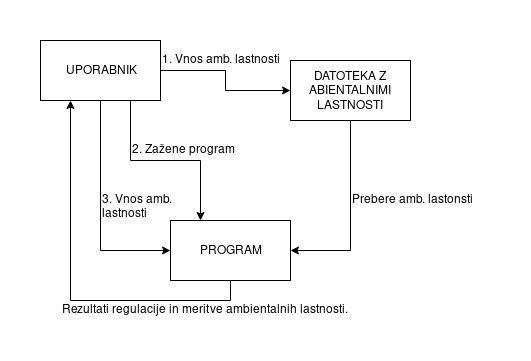
\includegraphics[width=15cm]{diagrami_slike/nivo_sistema.png}
						\end{figure}

					\newpage

					\item Slika 2 Nivo podsistemov - Diagram poteka.	

						\begin{figure}[h]
							\centering
							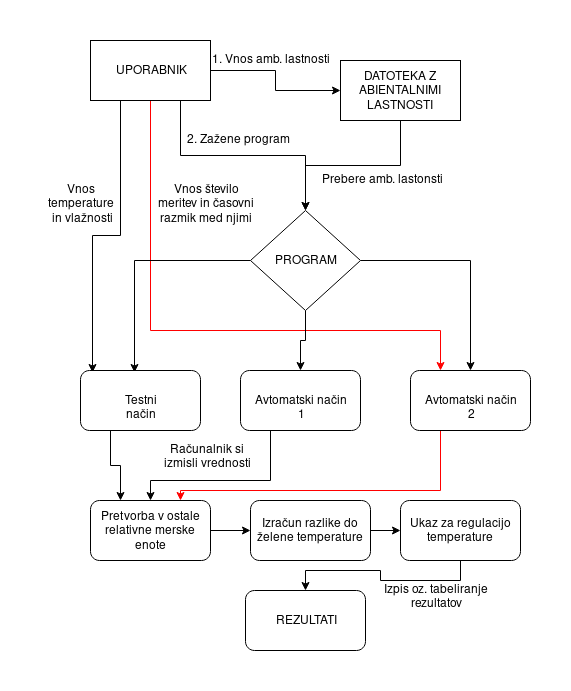
\includegraphics[width=13cm]{diagrami_slike/nivo_podsistemov.png}
						\end{figure}

				\end{itemize}
			
			\subsubsection{Opis procesov}
		
				\begin{itemize}
					\item Program - uporabnik zažene program in mu program omogoči izbiro med dvema načinoma delovanja programa
					\item Testni način - do testnega načina se lahko dostopi samo z argumentom -t ko se program zažene preko cmd.
						Testni način omogoča da uporabnik vnese temperaturo in vlažnost in na to avtmocki program nadaljue z izvajanjem
						ostalih izračunov.
					\item Avtomatski način 1 - izmisli vse potrebne veličine ki jih uporabnik vnaša v Testnem načinu oziroma simulira in
						na koncu prikaže rezultate pretvorb in izračunov.
					\item Avtomatski način 2 - uporabnik vnese število meritev in časovni razmik med njimi, ostale vrednosti program
						izmisli kot v Avtomatske načinu 1 in na koncu prikaže rezultate pretvorb in izračunov.
					\item Pretvorba v ostale relativne merske enote - program samo pretvori vneseno temperaturo v ostale merske enote.
					\item Izračun razlike do želene temperature - program izračuna razliko med vneseno temperaturo v programu 
						(dejanska temp. v prostoru) in želeno temperaturo ki jo prebere iz datoteke. Razlika temperature se izračuna
						v vseh enotah za temperaturo.
					\item Ukaz za regulacijo temperature - regulira temperaturo.
					\item Rezultati - rezultati so podani v obliki tabele.
				\end{itemize}


		\subsection{Opis podatkovnih tokov in terminatorjev}

			\subsubsection{Podatkovni slovar za sliko 2}

			\begin{center}
			\begin{tabular}{|c|c|c|c|c|c|}
					\hline 
					\rowcolor{purple!30!} &Ime podatka&Atribut&Tip&Veljavno območje&Opomba\\
					\hline
					1&Temperatura&&float&10 do 40&oblike: 14.36, 13.00\\
					\hline
					2&Vlažnost&&float&30 do 60&oblike: 42.5, 53.0\\
					\hline
					3&Število meritev&&integer&&\\
					\hline
					4&Časovni razmik&&integer&&\\
					\hline
			\end{tabular}
			\end{center}

			\subsubsection{Opis terminatorjev}
			{%\renewcommand{\arraystretch}{1.5}	
			\begin{center}
			\begin{tabular}{|c|c|}
					\hline
					\rowcolor{purple!30!}Ime terminatorja&Opomba \\
					\hline
					Uporabnik&Oseba ki uporablja program \\
					\hline
					Datoteka z ambientalnimi lastnosti & \thead{Vsaka ambientalna lastnost je napisana v novo vrstico \\ 
															Primer: TEMPERATURA: 25 \\ \hspace{0.7cm} VLAZNOST: 35 ...}  \\
					\hline
			\end{tabular}
			\end{center}
			}

		\subsection{Podroben opis in indeksiranje funkcij in drugih zahtev ki jih je potrebno implementirati}

			\subsubsection{Interaktivni vnos}
				\qquad \qquad Vnos temperature, vlažnosti, število meritev in časovni razmik preko tipkovnice.

			\subsubsection{Branje iz datoteke}
				\qquad \qquad Program mora znati prebrat ambientalne lastnosti iz datoteke.

			\subsubsection{Pretvorba temperature v ostale relativne merske enote}
				\qquad \qquad Program mora pretvoriti vneseno temperaturo v ostale merske enote za temperaturo.

			\subsubsection{Izračun razlike do želene temperature}
				\qquad \qquad Program mora izračunati razliko temperature v vseh mernih enotah.
			
			\subsubsection{Povprečna vrednost meritev in povprečno odstopanje}
				\qquad \qquad Program mora izračunati povprečno vrednost meritev ter povprečno odstopanje od 
				želenih vrednosti za posamezne parametre.

			\subsubsection{Tabeliranje rezultatov}
				\qquad \qquad Program mora tabelirati dobijenih rezultatov odvisnih od našega vnosa vrednosti.

			\subsubsection{Kontrola vhodnih podatkov}
				\qquad \qquad Program mora prepoznati in upozoriti če vnesemo ne veljavni tip podatka preko tipkovnice.

			\subsubsection{Testni način}
				\qquad \qquad Program mora imati vgrajen testni način delovanja ki je dostopen samo preko argumenta
				ki ga dodamo ko zaženemo program. Testni način nam omogoča vpis dodatnih podatkov za natačno testiranje.
		

		\subsection{Zunanji videz}

			\subsubsection{Glavni meni}

				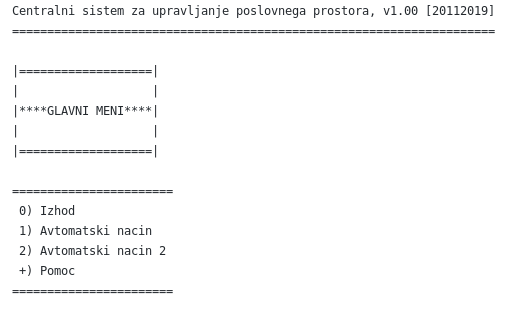
\includegraphics[width=11cm]{diagrami_slike/gl_meni.png}

			\subsubsection{Avtomatski način}

				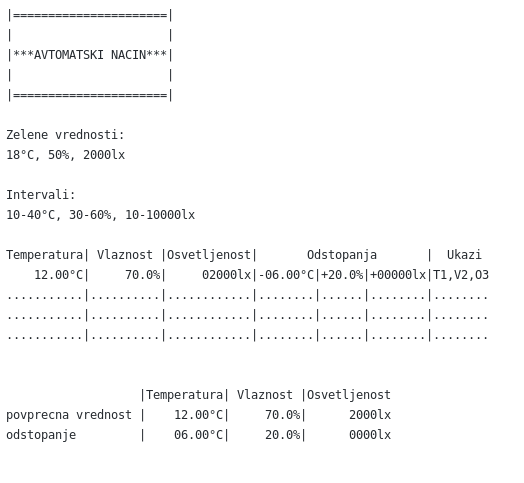
\includegraphics[width=11cm]{diagrami_slike/avt_nac.png}

\newpage

			\subsubsection{Avtomatski način 2}

				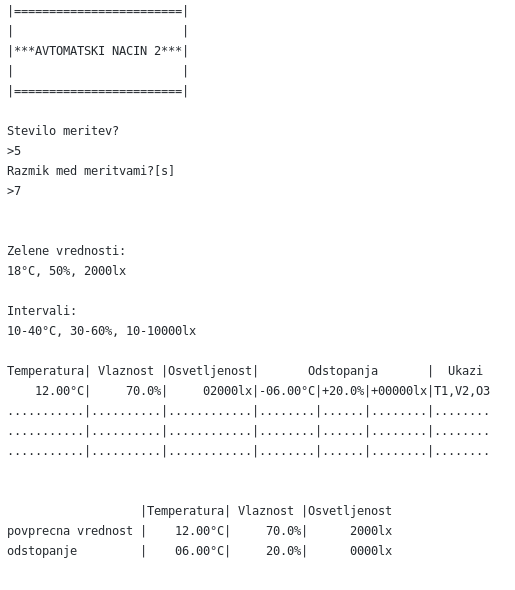
\includegraphics[width=10cm]{diagrami_slike/avt_nac2.png}

			\subsubsection{Pomoč}

				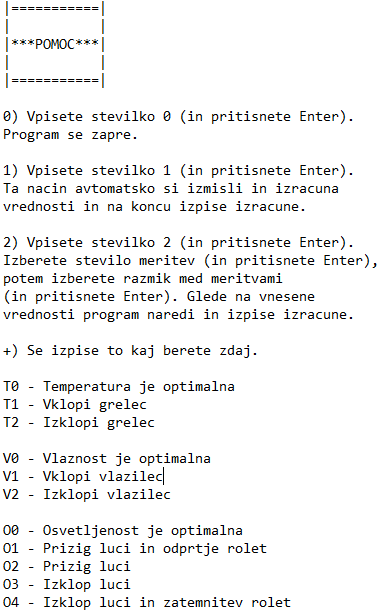
\includegraphics[width=7.3cm]{diagrami_slike/pomoc.png}

			\subsubsection{Testni način}
		
				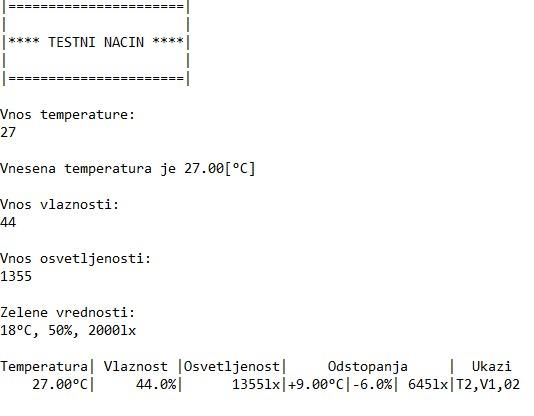
\includegraphics[width=8.2cm]{diagrami_slike/testni_nacin.jpg}

		\subsection{Opis funkcij, ki bodo najprej implementirane}

			\begin{itemize}
				\item Glavni meni
						\begin{itemize}
							\item Prebere vrednosti iz datoteke
							\item Interaktivna izbira načina delovanja
						\end{itemize}
				\item Avtomatski način
						\begin{itemize}
							\item Program si izmisli vrednosti
							\item Izračun odstopanja od želene vrednosti
							\item Ukaz za popravek
							\item Tabeliranje izračunane vrednosti
							\item Izračun povprečno vrednost meritev
							\item Izračun povprečno odstopanje od želenih vrednosti za posamezne parametre
						\end{itemize}
				\item Avtomatski način 2
						\begin{itemize}
							\item Interaktivni vnos za število meritev in časovni razmik med njimi
							\item Način izračuna in izpisa je enaki kot v Avtomatske načinu
						\end{itemize}
				\item Izhod
						\begin{itemize}
							\item Program se zapre
						\end{itemize}
			\end{itemize}

		\subsection{Prevzemni kriterij}

			\begin{itemize}
				\item Program mora biti dokumentiran skladno s standardom CVVS-2/2000
				\item Program mora biti preverjen na najmanj 15 testnih primerih. 
				Naročnik bo pripravil tri svoje testne primere, ki ne smejo pokazati na prisotnost večjih hib.
			\end{itemize}

\newpage

	\section{Testni primeri}

		\subsection{Povzetek}

		\qquad Na podlagi naročnikovih zahtev in Plana projekta, je bil izdelan ta dokument, ki natančno definira 
		postopek testiranja in testne primere. Dokument je  uporaben  za  evalvacijo  prototipa
		in  za  testiranje  kompletnega  programa.  Rezultati  testiranja  so  opisani 
		v Poročilu o preverjanju.

		\subsection{Identifikacija objektov, na katere se testni vzorci nanašajo}

		\qquad Testni primeri se nanašajo na csuppv0\_0\_20112019.exe in csuppv1\_0\_20112019.exe

		\subsection{Opis testnih primerov}

		\qquad Tvoreni so 17 testnih primerov v 3 kategorije, ki bodo za testiranje programa v1.0.

		\subsection{Opis testnega postopka}

		\qquad V okolju MS Windows odpremo datoteko v katro se nahaja program csuppvX\_Y\_DDMMYYYY.exe,
		z dvoklikom na miško zaženemo program in začnemo interaktivno vpisovati testne primere preko 
		tipkovnice. 

		\ V primeru testiranja testnega načina odpremo okno command prompt(cmd.exe) in z
		pomočjo ukaza \textbf{cd ime\_datoteke\textbackslash} se prestavimo v datoteko v katero se 
		nahaja csuppvX\_Y\_DDMMYYYY.exe in zaženemo program na način \textbf{csuppvX\_Y\_DDMMYYYY.exe -t}.

\newpage
	
	\begin{landscape}
		\subsection{Identifikacija funkcij in zahtev ter testna matrika}
			\footnotesize
			\centering
			\begin{tabular}{|c|c|c|c|c||c|c|c|c|c|c|c|c|c|c|c|c|c|c|c|c|c|c|c|c|}
			\hline
					Kratek opis&Kompleksnost&\thead{Stopnja \\  kritičnosti}&\thead{Indikator \\ pomembnosti}&\thead{Število \\ testov}
					&T&T&T&T&T&T&T&T&T&T&T&T&T&T&T&T&T&T&T&T\\
			\hline
				Interaktivni vnos&2&3&6&&&&&&&&&&&&&&&&&&&&&\\
				\hline
				Branje iz datoteke&2&3&6&&&&&&&&&&&&&&&&&&&&&\\
				\hline
				Pretvorba temp.&3&2&6&&&&&&&&&&&&&&&&&&&&&\\
				\hline
				Izračun temp. razl.&1&2&2&&&&&&&&&&&&&&&&&&&&&\\
				\hline
				PVM in PO&1&2&2&&&&&&&&&&&&&&&&&&&&&\\
				\hline
				Tabeliranje rezultov&2&2&4&&&&&&&&&&&&&&&&&&&&&\\
				\hline
				Kontrola vh. podat.&3&3&9&&&&&&&&&&&&&&&&&&&&&\\
				\hline
				Testni način&2&1&2&&&&&&&&&&&&&&&&&&&&&\\
				\hline
					Skupaj&&&37(100\%)&&&&&&&&&&&&&&&&&&&&&\\
			\hline

		\end{tabular}

	\end{landscape}
\newpage
		\subsection{Priloga}

			%\subsubsection{Opis vhodne domene}

			%\subsubsection{Opis izhodne domene}

			\subsubsection{Priloga s konkretnimi testni primeri}

			
			\ Preverjanje prisotnosti zahtev:
				\begin{itemize}

					\item TP1-1 Ali je prisotna najbolj kritična funkconalnost?
							Ali je implementiran testni režim?

					\item TP1-2 Ali je vedno prisotna vgrajena pomoč?

					%\item TP1-3 Ali sta zahtevana natančnost in hitrost prisotna?

				\end{itemize}
			\ Preverjanje natančnost in pravilnost izračunov:
				\begin{itemize}
					\item TP2-1 Ali program generira vse pravilne vrednosti za pravilno delovanje Avtomatskega načina?
					\item TP2-2 Ali program izvede zahtevano število meritev za zahtevanega časovnega rezmika ?
					\item TP2-3 Ali program izračuna povprečno vrednost meritev ter povprečno odstopanje od želenih vrednosti za posamezne parametre ?
					\item TP2-4 Ali program pretvori vneseno temperaturo v ostale merske enote ?
					\item TP2-5 Ali program izračuna razliko do želene temperature (v vseh merskih enotah) ?
					\item TP2-6 Ali program pravilno izvede ukaz za regulacijo temperature ?
					\item TP2-7 Ali program pravilno izračuna in izvede ukaze za vlažnost in osvetljenost ? 
					\item TP2-8 Ali program prekine svoje izvajanje na zahtevo uporabnika v Testnem načinu ?
				\end{itemize}
			\ Preverjanje robustnosti vhodnih podatkov:
				\begin{itemize}

					\item TP3-1 Ali program pravilno procesira neveljavne vhodne podatke?
					\item TP3-2 Ali program opozori za vnost temperature izven intervala $(10\ \degree C,40\ \degree C)$
					\item TP3-3 Ali program opozori za vnos vlažnosti izven intervala $(30\%,60\%)$
					\item TP3-4 Ali program opozori za vnos osvetljenosti izven intervala $(10\ lx,10000\ lx)$
					\item TP3-5 Ali program opozori za maksimalno možno število meritev?
					\item TP3-6 Ali program opozori za minimalni ali maksimalni časovni razmik med število meritev?
					\item TP3-7 Ali je program odporen na nepravilni vnos ambientalnih lastnosti v tekstovno datoteko?

				\end{itemize}
			
\newpage

	\begin{landscape}

			\paragraph{Ali je prisotna najbolj kritična funkcionalnost in Testni način ?}
			
			\centering
			
		
			\rowcolors{1}{purple!30!}{}
			\begin{tabular}{|c|c|c|c|}
			
					\hline
					Testni primer&Avtor&Verzija&Projekt \\
					\hline \hline
					TP1-1& Anton Zhezhov&V1.0&CSUPP \\
					\hline

			\end{tabular}
			
			\vspace{0.3cm}
			
			\rowcolors{1}{purple!30!}{}
			
			\begin{tabular}{|c|c|c|c|c|c|}
				\hline
				Začetno stanje&Namen&Konf. sistema&Strategija&Opomba&Odvisnost od drugih testov \\
				\hline \hline
				\thead{Okno Command Prompt \\ 
						(odprto na lokaciji \\
						mapao programa).}&\thead{Ali je prisotna najbolj \\ 
											kritična funkcionalnost \\ 
											in Testni način ?}& Windows 10 Pro&\thead{Preverjanje \\ 
																						prisotnosti zahtev.}&\thead{Testni način \\ 
																											je za demonstracijo
																											\\delovanje programa.}&Ni nobene odvisnosti. \\
				\hline
			\end{tabular}

			\vspace{0.3cm}

			\rowcolors{1}{purple!30!}{}
			
			\begin{tabular}{|c|c|c|C{5.5cm}|c|c|}
					\hline
					Korak&Akcija/Ime vhodne spremenjljivke&Vrednost&Pričekovana reakcija/vrednost&Opomba&Opomba za testno poročilo \\
					\hline \hline
					1&csuppvX\_Y\_DDMMYYYY.exe -t&&\small{Izpis da smo v Testnem  
														načinu, pod izpisa, interaktivni 
														vnos za temeraturo.}&&\\
					\hline
					2&Vpišemo temperaturo&37&\small{Izpis vnesene temperature   
													z enoto in pretvorba v ostale merske 
													enote, pod izpisa, 
													interaktivni vnost za vlažnost.}&&\\
					3&Vpišemo vlažnost&48&\small{Pod vpisano vrednost,
												interaktivni vnost za osvetljenost.}&&\\
					\hline
					4&Vpišemo osvetljenost&5243&\small{Pod vpisano vrednost se izpišejo
													želene vrednosti se izvedejo 
													potrebni izračuni in tabeliranje.}&&\\
					\hline
					5&Zahtevamo prekinitev izračunov&p&Izračuni in tabeliranje se prekineta.&&\\

					\hline
					6&Izberemo ponovni vnos vrednosti&*&\small{Izpis da smo v Testnem 
														načinu, pod izpisa, interaktivni 
														vnos za temeraturo.}&&\\
					\hline
					7&Korake od 2 do 5&&\small{Pričekujemo enaki 
										način delovanje
										kot v korake od 2 do 5.}&&\\ 
					\hline
					8&Želimo izhod&0&\small{Okno Command Prompt
											(odprto na lokaciji
											mapao programa).}&&\\
					\hline
			\end{tabular}


			
	\end{landscape}

\newpage

	\begin{landscape}
	
		\paragraph{Ali je vedno prisotna vgrajena pomoč ?}
			
			\centering
			
		
			\rowcolors{1}{purple!30!}{}
			\begin{tabular}{|c|c|c|c|}
			
					\hline
					Testni primer&Avtor&Verzija&Projekt \\
					\hline \hline
					TP1-2& Anton Zhezhov&V1.0&CSUPP \\
					\hline

			\end{tabular}
			
			\vspace{0.3cm}
			
			\rowcolors{1}{purple!30!}{}
			
			\begin{tabular}{|c|c|c|c|c|c|}
				\hline
				Začetno stanje&Namen&Konf. sistema&Strategija&Opomba&Odvisnost od drugih testov \\
				\hline \hline
				\thead{Okno Command Prompt \\ 
						(odprto na lokaciji \\
						mapao programa).}&\thead{Ali je vedno prisotna \\ 
											vgrajena pomoč ? \\}& Windows 10 Pro&\thead{Preverjanje \\ 
																						prisotnosti zahtev.}&\thead{Testni način \\ 
																											je za demonstracijo
																											\\delovanje programa.}&Ni nobene odvisnosti. \\
				\hline
			\end{tabular}

			\vspace{0.3cm}

			\rowcolors{1}{purple!30!}{}

			\begin{tabular}{|c|c|c|C{5.5cm}|c|c|}
					\hline
					Korak&Akcija/Ime vhodne spremenjljivke&Vrednost&Pričekovana reakcija/vrednost&Opomba&Opomba za testno poročilo \\
					\hline \hline
					1&csuppvX\_Y\_DDMMYYYY.exe -t&&\small{Izpis da smo v Testnem  
														načinu, pod izpisa, interaktivni 
														vnos za temeraturo.}&&\\
					\hline
					2&Zahtevamo pomoč&+&Izpis pomoči za to polje&&\\
					\hline
					3&Vpišemo temperaturo&37&\small{Izpis vnesene temperature   
													z enoto in pretvorba v ostale merske enote, 
													pod izpisa, 
													interaktivni vnost za vlažnost.}&&\\
					\hline
					4&Zahtevamo pomoč&+&Izpis pomoči za to polje&&\\
					\hline
					5&Vpišemo vlažnost&48&\small{Pod vpisano vrednost,
												interaktivni vnost za osvetljenost.}&&\\
					\hline
					6&Zahtevamo pomoč&+&Izpis pomoči za to polje&&\\
					\hline
					7&Vpišemo osvetljenost&5243&\small{Pod vpisano vrednost se izpišejo
													želene vrednosti se izvedejo 
													potrebni izračuni in tabeliranje.}&&\\
					\hline
					8&Zahtevamo pomoč&+&Izpis pomoči za to polje&&\\
					\hline
					9&Izberemo ponovni vnos vrednosti&*&\small{Izpis da smo v Testnem 
														načinu, pod izpisa, interaktivni 
														vnos za temeraturo.}&&\\
					\hline
					10&Korake od 2 do 9&&\small{Pričekujemo enaki 
										način delovanje
										kot v korake od 2 do 9.}&&\\ 
					\hline
					11&Želimo izhod&0&\small{Okno Command Prompt
											(odprto na lokaciji
											mapao programa).}&&\\
					\hline
			\end{tabular}

	\end{landscape}

\newpage

	\begin{landscape}
	
		\paragraph{Ali program generira vse pravilne vrednosti za pravilno delovanje Avtomatskega načina ?}
			
			\centering
			
		
			\rowcolors{1}{purple!30!}{}
			\begin{tabular}{|c|c|c|c|}
			
					\hline
					Testni primer&Avtor&Verzija&Projekt \\
					\hline \hline
					TP2-1& Anton Zhezhov&V1.0&CSUPP \\
					\hline

			\end{tabular}
			
			\vspace{0.3cm}
			
			\rowcolors{1}{purple!30!}{}
			
			\begin{tabular}{|c|c|c|c|c|c|}
				\hline
				Začetno stanje&Namen&Konf. sistema&Strategija&Opomba&Odvisnost od drugih testov \\
				\hline \hline
				\thead{Okno Command Prompt \\ 
						(odprto na lokaciji \\
						mapao programa).}&\thead{Generiranje \\  
												pravilne vrednosti.}& Windows 10 Pro&\thead{Preverjanje natančnost \\  
																						 in pravilnost.}&Ni opomb.&Ni nobene odvisnosti. \\
				\hline
			\end{tabular}

			\vspace{0.3cm}

			\rowcolors{1}{purple!30!}{}

			\begin{tabular}{|c|c|c|C{5.5cm}|c|c|}
					\hline
					Korak&Akcija/Ime vhodne spremenjljivke&Vrednost&Pričekovana reakcija/vrednost&Opomba&Opomba za testno poročilo \\
					\hline \hline
					1&csuppvX\_Y\_DDMMYYYY.exe&&\small{Izpis da smo v Glavni meni,  
														pod izpisom, interaktivni
														vnos za izbiro načina delovanja.}&&\\
					\hline
					2&Izberemo Avtomatski način&1&\small{Izpis da smo v Avtomatskem
													načinu, izpis želenih vrednost, 
													izpis intervalov, tabeliranje, 
													izpis povprečne vrednosti in odstopanje.}&&\\
					\hline
					3&Izberemo Avtomatski način &1&\small{Pričekujemo enaki izpis kot prej.}&&\\
					
					\hline
					4&Zahtevamo izhod&0&Okno Command Prompt
										(odprto na lokaciji 
										mapao programa).&&\\
					\hline
			\end{tabular}

	\end{landscape}

\newpage

	\begin{landscape}
	
		\paragraph{Ali program izvede zahtevano število meritev za zahtevanega časovnega razmika ?}
			
			\centering
			
		
			\rowcolors{1}{purple!30!}{}
			\begin{tabular}{|c|c|c|c|}
			
					\hline
					Testni primer&Avtor&Verzija&Projekt \\
					\hline \hline
					TP2-2& Anton Zhezhov&V1.0&CSUPP \\
					\hline

			\end{tabular}
			
			\vspace{0.3cm}
			
			\rowcolors{1}{purple!30!}{}
			
			\begin{tabular}{|c|c|c|c|c|c|}
				\hline
				Začetno stanje&Namen&Konf. sistema&Strategija&Opomba&Odvisnost od drugih testov \\
				\hline \hline
				\thead{Okno Command Prompt \\ 
						(odprto na lokaciji \\
						mapao programa).}&\thead{Število meritev in\\  
												časovni razmik.}& Windows 10 Pro&\thead{Preverjanje natančnost \\  
																						 in pravilnost.}&Ni opomb.&Ni nobene odvisnosti. \\
				\hline
			\end{tabular}

			\vspace{0.3cm}

			\rowcolors{1}{purple!30!}{}

			\begin{tabular}{|c|c|c|C{5.5cm}|c|c|}
					\hline
					Korak&Akcija/Ime vhodne spremenjljivke&Vrednost&Pričekovana reakcija/vrednost&Opomba&Opomba za testno poročilo \\
					\hline \hline
					1&csuppvX\_Y\_DDMMYYYY.exe&&\small{Izpis da smo v Glavni meni,  
														pod izpisom, interaktivni
														vnos za izbiro načina delovanja.}&&\\
					\hline
					2&Izberemo Avtomatski način&1&\small{Izpis da smo v Avtomatskem
													načinu, izpis želenih vrednost, 
													izpis intervalov, tabeliranje, 
													izpis povprečne vrednosti in odstopanje.}&&\\
					\hline
					3&Izberemo Avtomatski način &1&\small{Pričekujemo enaki izpis kot prej
															in 100 meritve na vsake 3 sekunde v tabelo.}&&\\
					
					\hline
					4&Zahtevamo izhod&0&Okno Command Prompt
										(odprto na lokaciji 
										mapao programa).&&\\
					\hline
			\end{tabular}

	\end{landscape}

\newpage

	\begin{landscape}
	
		\paragraph{Ali program izračuna povprečno vrednost meritev ter povprečno odstopanje od želenih vrednosti za posamezne parametre ?}
			
			\centering
			
		
			\rowcolors{1}{purple!30!}{}
			\begin{tabular}{|c|c|c|c|}
			
					\hline
					Testni primer&Avtor&Verzija&Projekt \\
					\hline \hline
					TP2-3& Anton Zhezhov&V1.0&CSUPP \\
					\hline

			\end{tabular}
			
			\vspace{0.3cm}
			
			\rowcolors{1}{purple!30!}{}
			
			\begin{tabular}{|c|c|c|c|c|c|}
				\hline
				Začetno stanje&Namen&Konf. sistema&Strategija&Opomba&Odvisnost od drugih testov \\
				\hline \hline
				\thead{Okno Command Prompt \\ 
						(odprto na lokaciji \\
						mapao programa).}&\thead{Povprečna vrednost meritev \\  
												in povprečno odstopanje.}& Windows 10 Pro&\thead{Preverjanje natančnost \\  
																						 in pravilnost.}&Ni opomb.&Ni nobene odvisnosti. \\
				\hline
			\end{tabular}

			\vspace{0.3cm}

			\rowcolors{1}{purple!30!}{}

			\begin{tabular}{|c|c|c|C{5.5cm}|c|c|}
					\hline
					Korak&Akcija/Ime vhodne spremenjljivke&Vrednost&Pričekovana reakcija/vrednost&Opomba&Opomba za testno poročilo \\
					\hline \hline
					1&csuppvX\_Y\_DDMMYYYY.exe&&\small{Izpis da smo v Glavni meni,  
														pod izpisom, interaktivni
														vnos za izbiro načina delovanja.}&&\\
					\hline
					2&Izberemo Avtomatski način&1&\small{Izpis da smo v Avtomatskem
													načinu, izpis želenih vrednost, 
													izpis intervalov, tabeliranje, 
													izpis povprečne vrednosti in odstopanje.}&&\\
					\hline
					3&Izberemo Avtomatski način &1&\small{Pričekujemo enaki izpis kot prej
															in po tabeli izpis povprečne 
															vrednosti in odstopanje za
															Temp., Vlaž. in Osvetljenost.}&&\\
					
					\hline
					4&Zahtevamo izhod&0&Okno Command Prompt
										(odprto na lokaciji 
										mapao programa).&&\\
					\hline
			\end{tabular}
	\end{landscape}

\newpage

	\begin{landscape}
	
		\paragraph{Ali program pretvori vneseno temperaturo v ostale merske enote ?}
			
			\centering
			
		
			\rowcolors{1}{purple!30!}{}
			\begin{tabular}{|c|c|c|c|}
			
					\hline
					Testni primer&Avtor&Verzija&Projekt \\
					\hline \hline
					TP2-4& Anton Zhezhov&V1.0&CSUPP \\
					\hline

			\end{tabular}
			
			\vspace{0.3cm}
			
			\rowcolors{1}{purple!30!}{}
			
			\begin{tabular}{|c|c|c|c|c|c|}
				\hline
				Začetno stanje&Namen&Konf. sistema&Strategija&Opomba&Odvisnost od drugih testov \\
				\hline \hline
				\thead{Okno Command Prompt \\ 
						(odprto na lokaciji \\
						mapao programa).}&\thead{Pretvorba temperature \\  
												v ostale merske enote.}& Windows 10 Pro&\thead{Preverjanje natančnost \\  
																						 in pravilnost.}&Ni opomb.&Ni nobene odvisnosti. \\
				\hline
			\end{tabular}

			\vspace{0.3cm}

			\rowcolors{1}{purple!30!}{}

			\begin{tabular}{|c|c|c|C{5.9cm}|c|c|}
					\hline
					Korak&Akcija/Ime vhodne spremenjljivke&Vrednost&Pričekovana reakcija/vrednost&Opomba&Opomba za testno poročilo \\
					\hline \hline
					1&csuppvX\_Y\_DDMMYYYY.exe -t&&\small{Izpis da smo v Testni način,  
														pod izpisom, interaktivni
														vnos za temperaturo.}&&\\
					\hline
					2&Vpišemo temperaturo&300.15&\small{Izpis da je vnesena 
														temperatura 300.15[K] in izpis
														pretvorbe v ostale merske enote, potem
														vnos nadaljuje kot v TP1-1 od koraka 3.}&&\\
					\hline
					3&Vpišemo temperaturo&308.15&\small{Izpis da je vnesena 
														temperatura 308.15[K] in izpis
														pretvorbe v ostale merske enote, potem
														vnos nadaljuje kot v TP1-1 od koraka 3.}&&\\

					\hline
					4&Zahtevamo izhod&0&Okno Command Prompt
										(odprto na lokaciji 
										mapao programa).&&\\
					\hline
			\end{tabular}
	\end{landscape}

\newpage

	\begin{landscape}
	
		\paragraph{Ali program izračuna razliko do želene temperature ?}
			
			\centering
			
		
			\rowcolors{1}{purple!30!}{}
			\begin{tabular}{|c|c|c|c|}
			
					\hline
					Testni primer&Avtor&Verzija&Projekt \\
					\hline \hline
					TP2-5& Anton Zhezhov&V1.0&CSUPP \\
					\hline

			\end{tabular}
			
			\vspace{0.3cm}
			
			\rowcolors{1}{purple!30!}{}
			
			\begin{tabular}{|c|c|c|c|c|c|}
				\hline
				Začetno stanje&Namen&Konf. sistema&Strategija&Opomba&Odvisnost od drugih testov \\
				\hline \hline
				\thead{Okno Command Prompt \\ 
						(odprto na lokaciji \\
						mapao programa).}&\thead{Izračun razlike do\\  
											želene temperature.}& Windows 10 Pro&\thead{Preverjanje natančnost \\  
																						 in pravilnost.}&Ni opomb.&Ni nobene odvisnosti. \\
				\hline
			\end{tabular}

			\vspace{0.3cm}

			\rowcolors{1}{purple!30!}{}

			\begin{tabular}{|c|c|c|C{5.9cm}|c|c|}
					\hline
					Korak&Akcija/Ime vhodne spremenjljivke&Vrednost&Pričekovana reakcija/vrednost&Opomba&Opomba za testno poročilo \\
					\hline \hline
					1&csuppvX\_Y\_DDMMYYYY.exe -t&&\small{Izpis da smo v Testni način,  
														pod izpisom, interaktivni
														vnos za temperaturo.}&&\\
					\hline
					2&Vpišemo temperaturo&300.15&\small{Izpis da je vnesena 
														temperatura 300.15[K] in izpis
														pretvorbe v ostale merske enote, potem
														vnos nadaljuje kot v TP1-1 koraka 3 in 4 in 
														se izpiše tabela z izračunane razlike .}&&\\
					\hline
					3&Vpišemo temperaturo&308.15&\small{Izpis da je vnesena 
														temperatura 308.15[K] in izpis
														pretvorbe v ostale merske enote, potem
														vnos nadaljuje kot v TP1-1 koraka 3 in 4 in 
														se izpiše tabela z izračunane razlike.}&&\\

					\hline
					4&Zahtevamo izhod&0&Okno Command Prompt
										(odprto na lokaciji 
										mapao programa).&&\\
					\hline
			\end{tabular}
	\end{landscape}

\newpage

	\begin{landscape}
	
		\paragraph{Ali program pravilno izvede ukaze za regulacijo ?}
			
			\centering
			
		
			\rowcolors{1}{purple!30!}{}
			\begin{tabular}{|c|c|c|c|}
			
					\hline
					Testni primer&Avtor&Verzija&Projekt \\
					\hline \hline
					TP2-6& Anton Zhezhov&V1.0&CSUPP \\
					\hline

			\end{tabular}
			
			\vspace{0.3cm}
			
			\rowcolors{1}{purple!30!}{}
			
			\begin{tabular}{|c|c|c|c|c|c|}
				\hline
				Začetno stanje&Namen&Konf. sistema&Strategija&Opomba&Odvisnost od drugih testov \\
				\hline \hline
				\thead{Okno Command Prompt \\ 
						(odprto na lokaciji \\
						mapao programa).}&\thead{Ukazi za \\  
											regulacijo temperature.}& Windows 10 Pro&\thead{Preverjanje natančnost \\  
																						 in pravilnost.}&Ni opomb.&Ni nobene odvisnosti. \\
				\hline
			\end{tabular}

			\vspace{0.3cm}

			\rowcolors{1}{purple!30!}{}

			\begin{tabular}{|c|c|c|C{5.9cm}|c|c|}
					\hline
					Korak&Akcija/Ime vhodne spremenjljivke&Vrednost&Pričekovana reakcija/vrednost&Opomba&Opomba za testno poročilo \\
					\hline \hline
					1&csuppvX\_Y\_DDMMYYYY.exe &&\small{Izpis da smo v Glavni meni,  
														pod izpisom, interaktivni
														vnos za izbiro načina delovanja.}&&\\
					\hline
					2&Izberemo Avtomatski način&1&\small{Enako delovanje kot v primer 
														TP2-1 korak 2 in pričekujemo 
														ukaze za regulacijo v najbolj desnem stolpcu tabele.}&&\\
					\hline
					3&Zahtevamo izhod&0&Okno Command Prompt
										(odprto na lokaciji 
										mapao programa).&&\\
					\hline
			\end{tabular}
	\end{landscape}

\newpage

	\begin{landscape}
	
		\paragraph{Ali program pravilno izvede ukaze za vlažnost in osvetljenost ?}
			
			\centering
			
		
			\rowcolors{1}{purple!30!}{}
			\begin{tabular}{|c|c|c|c|}
			
					\hline
					Testni primer&Avtor&Verzija&Projekt \\
					\hline \hline
					TP2-7& Anton Zhezhov&V1.0&CSUPP \\
					\hline

			\end{tabular}
			
			\vspace{0.3cm}
			
			\rowcolors{1}{purple!30!}{}
			
			\begin{tabular}{|c|c|c|c|c|c|}
				\hline
				Začetno stanje&Namen&Konf. sistema&Strategija&Opomba&Odvisnost od drugih testov \\
				\hline \hline
				\thead{Okno Command Prompt \\ 
						(odprto na lokaciji \\
						mapao programa).}&\thead{Ukazi za regulacijo\\  
											valžnosti in osvetljenosti.}& Windows 10 Pro&\thead{Preverjanje natančnost \\  
																						 in pravilnost.}&Ni opomb.&Ni nobene odvisnosti. \\
				\hline
			\end{tabular}

			\vspace{0.3cm}

			\rowcolors{1}{purple!30!}{}

			\begin{tabular}{|c|c|c|C{5.9cm}|c|c|}
					\hline
					Korak&Akcija/Ime vhodne spremenjljivke&Vrednost&Pričekovana reakcija/vrednost&Opomba&Opomba za testno poročilo \\
					\hline \hline
					1&csuppvX\_Y\_DDMMYYYY.exe &&\small{Izpis da smo v Glavni meni,  
														pod izpisom, interaktivni
														vnos za izbiro načina delovanja.}&&\\
					\hline
					2&Izberemo Avtomatski način&1&\small{Enako delovanje kot v primer 
														TP2-1 korak 2 in pričekujemo 
														ukaze za regulacijo v najbolj desnem stolpcu tabele.}&&\\
					\hline
					3&Zahtevamo izhod&0&Okno Command Prompt
										(odprto na lokaciji 
										mapao programa).&&\\
					\hline
			\end{tabular}
	\end{landscape}

\newpage

	\begin{landscape}
	
		\paragraph{Ali program prekine svoje izvajanje na zahtevo uporabnika v Testnem načinu ?}
			
			\centering
			
			\rowcolors{1}{purple!30!}{}
			\begin{tabular}{|c|c|c|c|}
			
					\hline
					Testni primer&Avtor&Verzija&Projekt \\
					\hline \hline
					TP2-8& Anton Zhezhov&V1.0&CSUPP \\
					\hline

			\end{tabular}
			
			\vspace{0.3cm}
			
			\rowcolors{1}{purple!30!}{}
			
			\begin{tabular}{|c|c|c|c|c|c|}
				\hline
				Začetno stanje&Namen&Konf. sistema&Strategija&Opomba&Odvisnost od drugih testov \\
				\hline \hline
				\thead{Okno Command Prompt \\ 
						(odprto na lokaciji \\
						mapao programa).}&\thead{Prekinitev \\  
											izvajanja.}& Windows 10 Pro&\thead{Preverjanje natančnost \\  
																						 in pravilnost.}&Ni opomb.&Ni nobene odvisnosti. \\
				\hline
			\end{tabular}

			\vspace{0.3cm}

			\rowcolors{1}{purple!30!}{}

			\begin{tabular}{|c|c|c|C{5.9cm}|c|c|}
					\hline
					Korak&Akcija/Ime vhodne spremenjljivke&Vrednost&Pričekovana reakcija/vrednost&Opomba&Opomba za testno poročilo \\
					\hline \hline
					1&csuppvX\_Y\_DDMMYYYY.exe -t &&\small{Izpis da smo v Testni način,  
														pod izpisom, interaktivni
														vnos za temperaturo.}&&\\
					\hline
					2&Vnesemo temperaturo&30&\small{Enako delovanje kot v primer 
														TP1-1 od koraka 2 do koraka 4.}&&\\
					\hline
					3&Zahtevamo prekinitev izračunov&p&Izračuni in tabeliranje se prekineta.&&\\
					\hline
					4&Zahtevamo izhod&0&Okno Command Prompt
										(odprto na lokaciji 
										mapao programa).&&\\
					\hline
			\end{tabular}
	\end{landscape}

\newpage

	\begin{landscape}
	
			\paragraph{Procesiranje neveljavnih vhodnih podatkov (od TP3-1 do TP3-6).}
			
			\centering
			
			\rowcolors{1}{purple!30!}{}
			\begin{tabular}{|c|c|c|c|}
			
					\hline
					Testni primeri&Avtor&Verzija&Projekt \\
					\hline \hline
					TP3-1 do TP3-6& Anton Zhezhov&V1.0&CSUPP \\
					\hline

			\end{tabular}
			
			\vspace{0.3cm}
			
			\rowcolors{1}{purple!30!}{}
			
			\begin{tabular}{|c|c|c|c|c|c|}
				\hline
				Začetno stanje&Namen&Konf. sistema&Strategija&Opomba&Odvisnost od drugih testov \\
				\hline \hline
				\thead{Okno Command Prompt \\ 
						(odprto na lokaciji \\
						mapao programa).}&\thead{Procesiranje \\  
											neveljavnih podatkov.}& Windows 10 Pro&\thead{Preverjanje robustnosti \\  
																						 vhodnih podatkov.}&Ni opomb.&Ni nobene odvisnosti. \\
				\hline
			\end{tabular}

			\vspace{0.3cm}

			\rowcolors{1}{purple!30!}{}

			\begin{tabular}{|c|c|c|C{10cm}|c|c|}
					\hline
					Korak&Akcija/Ime vhodne spremenjljivke&Vrednost&Pričekovana reakcija/vrednost&Opomba&OTP \\
					\hline \hline
					1&csuppvX\_Y\_DDMMYYYY.exe -t &&\small{Izpis da smo v Testni način,  
														pod izpisom, interaktivni
														vnos za temperaturo.}&&\\
					\hline
					2&Vnesemo temperaturo&-120000.12&\small{Opozotilo za neveljavno vrednost 
														temperature, potem se pojavi ponovni 
														interaktivni vnos za temperaturo.}&&\\
					\hline
					3&Vnesemo vlažnost &172.8&\small{Opozotilo za neveljavno vrednost 
														vlažnsti, potem se pojavi ponovni 
														interaktivni vnos za vlažnost.}&&\\
					\hline
					4&Vnesemo osvetljenost &-127a&\small{Opozotilo za neveljavno vrednost 
														osvetljenosti, potem se pojavi ponovni 
														interaktivni vnos za osvetljenost.}&&\\
					\hline
					5&Zahtevamo prekinitev izračunov&p&Izračuni in tabeliranje se prekineta.&&\\
					\hline
					6&Zahtevamo izhod&0&Okno Command Prompt
										(odprto na lokaciji 
										mapao programa).&&\\
					\hline
					7&csuppvX\_Y\_DDMMYYYY.exe&&\small{Izpis da smo v Glavni meni,  
														pod izpisom, interaktivni
														vnos za izbiro načina delovanja.}&&\\
					\hline
					8&Izberemo Avtomatski način 2&2&\small{Izpis za interaktivni vnost število
															meritev.}&&\\
					\hline
					9&Vpišemo število meritev&10.23e-18&\small{Opozorilo za neveljavno vrednost
																meritve, potem se pojavi ponovni 
																interaktivni vnos za številio meritve.}&&\\
					\hline
					10&Vpišemo časovni razmik&65*87&\small{Opozorilo za neveljavno vrednost
															razmika, potem se pojavi ponovni 
															interaktivni vnos za časovni razmik in tabeliranje.}&&\\
					\hline
					11&Zahtevamo ponovno izbiro načina delovanja&¸&\small{Opozorilo za neveljavno vrednost za izbor načina 
																		delovanja, potem se pojavi ponovni 
																		interaktivni vnos za izbiro.}&&\\
					\hline
					12&Zahtevamo izhod&ž&\small{Opozorilo za neveljavno komando za izhod, potem se 
												program vrne v prejšno stanje v kero je bil.} &&\\
					\hline
					13&Zahtevamo izhod&0&Okno Command Prompt
										(odprto na lokaciji 
										mapao programa).&&\\
					\hline
			\end{tabular}
	\end{landscape}

\newpage

	\begin{landscape}
	
			\paragraph{Ali je program odporen na nepravilni vnos ambientalnih lastnosti v datoteki ?}
			
			\centering
			
			\rowcolors{1}{purple!30!}{}
			\begin{tabular}{|c|c|c|c|}
			
					\hline
					Testni primer&Avtor&Verzija&Projekt \\
					\hline \hline
					TP3-7& Anton Zhezhov&V1.0&CSUPP \\
					\hline

			\end{tabular}
			
			\vspace{0.3cm}
			
			\rowcolors{1}{purple!30!}{}
			
			\begin{tabular}{|c|c|c|c|c|c|}
				\hline
				Začetno stanje&Namen&Konf. sistema&Strategija&Opomba&Odvisnost od drugih testov \\
				\hline \hline
				\thead{Okno Command Prompt \\ 
						(odprto na lokaciji \\
						mapao programa).}&\thead{Procesiranje \\  
											neveljavnih podatkov.}& Windows 10 Pro&\thead{Preverjanje robustnosti \\  
																						 vhodnih podatkov.}&Ni opomb.&Ni nobene odvisnosti. \\
				\hline
			\end{tabular}

			\vspace{0.3cm}

			\rowcolors{1}{purple!30!}{}

			\begin{tabular}{|c|c|c|C{10cm}|c|c|}
					\hline
					Korak&Akcija/Ime vhodne spremenjljivke&Vrednost&Pričekovana reakcija/vrednost&Opomba&OTP \\
					\hline \hline
					1&csuppvX\_Y\_DDMMYYYY.exe -t &&\small{Izpis da smo v Testni način,  
														pod izpisom opozorilo da 
														tekstovna datoteka vsebuje neveljavni tip  podatkov.}&&\\
					\hline
					2&csuppvX\_Y\_DDMMYYYY.exe&&\small{Izpis da smo v Glavni meni,  
														pod izpisom, opozorilo da tekstovna datoteka vsebuje
														neveljavni tip podatkov.}&&\\
					\hline
			\end{tabular}
	\end{landscape}

\newpage

\section{Poročilo o preverjanju}

	\subsection{Povzetek}

	\qquad Program smo preverili v skladu s standardom CVVS 2-2000. Za testiranje 
			programa smo uporabili testne primere opisane v točki: Testni primeri.

	\subsection{Izvedene aktivnosti in ugotovitve}
	
		\subsubsection{Splošni pregled vmesnih dokumentov oziroma produktov}
		
		\subsubsection{Evalvacija prototipa}

		\qquad Vse nepravilnosti prototipa glede stila kodiranja in nepravilno 
				delovanje programa so bile ustno sporočene razvijalcu. Za testiranje
				prototipa sta bila uporabljena testna primera TP2-2 in TP2-3.
		
		\subsubsection{Pregled izvorne kode}
	
		\qquad Informacije od programa za kompleksnost

		\subsubsection{Testiranje končnega produkta}

		\qquad Testiranje je potekalo na računalniku s Windows 10 Pro. Testirali smo 
		verzijo v1.0 in v2.0 programa.

		\vspace{0.5cm}

		\hspace{-0.8cm} \qquad {\bf{Uporabljene strategije:}} 

		\begin{itemize}
			\item Prisotnost zahtev
			\item Preverjanje robustnosti
			\item Ugibanje nepravilnosti
			\item Mejne vrednosti
		\end{itemize}
		
		\hspace{-0.8cm} \qquad {\bf{Vložen napor:}}
		
		\vspace{0.3cm}

		\qquad Glede na izbrane strategije smo uporabili 12 testnih primerov 
				ki so opisani v točko: Testni primeri.

		\vspace{0.5cm}

		\hspace{-0.8cm} \qquad {\bf{Dosežena temeljitost:}}
		
		\vspace{0.3cm}

		\qquad Planirana terminalna kriterijska funkcija.  S  testiranjem  končamo ko sta izpolnjena pogoja a in b  alipogoj c:

			\begin{enumerate}[label=\alph*]
					\item) Preveriti je potrebno prisotnost vseh zahtev, ki so podane v sistemskih specifikacijah.
					\item) Vsaka funkcija v izvorni kodi mora biti klicana najmanj enkrat.
					\item) Ko preteče predvideno obdobje, ki je namenjeno testiranju.
			\end{enumerate}

\newpage

		\qquad Dosežena pokritost kode:

			\begin{itemize}
				\item Nepokritost zahteve za progran v1.0:

				\qquad Po izračunu ni bilo mogoče izbrati ponovni vnos za keri bilo način delovanja razen Testnega načina. 

				\item Nepokritost zahteve za program v2.0:
			
				\qquad Pri izbor Avtomatski način 2 program javi napako in se program zapre.
			\end{itemize}


		\vspace{0.5cm}

		\hspace{-0.8cm} \qquad {\bf{Ugotovitve:}}
		
		\vspace{0.3cm}

		\qquad V prvi verziji programa (v1.0) je bilo odkritih 7 nepravilnosti. Od tega je 
				razvojna oseba takoj odpravila 2 nepravilnosti. Eno nepravilnost je razvojna
				oseba predstavila za drugo verzijo programa (v2.0). 

		\qquad	Zaradi opravičenih razlogov razvojna oseba ni uspela do konca odpraviti napake 
		iz prve verzije programa (v1.0) in se je odločila da več ne bo sodelovala v projektu. 
		To ima vpliv na drugo verzijo programa in to pomeni da druga verzija programa ni dokončana.

\newpage

	\begin{landscape}

	\subsection{Poročilo o najdenih nepravilnostih}

		\centering

			\rowcolors{1}{purple!30!}{}
			\begin{tabular}{|c|C{3cm}|C{8cm}|c|c|c|c|}
				
					\hline
					Nepravilnost & Testni primer & Opis nepravilnosti & Resnost & Verzija & Končni status & Opomba \\
					\hline
					1/1&TP2-1&Ni omogočen ponovni izbir načina delovanja& 2 & v1.0 & Odpravljeno v v2.0& \\
					\hline
					1/2&TP3-1 - TP3-6 
						Korak 1 - 6&Neskončna zanka pri neveljavni vnos& 3 & v1.0 & Ni odpravljeno& \\
					\hline
					1/3&TP2-4&Ne zaznava enot temperature iz datoteke & 3 & v1.0 & Ni odpravljeno& \\
					\hline
					1/4&TP2-2&Čas. razmik med meritvami je manj kot 3s& 2 & v1.0 & Odpravljeno v v2.0& \\
					\hline
					1/5&TP3-5&Ne dobimo upozorilo za max. ali min. število 
								meritev ali max. ali min čas. razmik& 2 & v1.0 & Ni odpravljeno& \\
					\hline
					1/6&TP3-1 - TP3-6  
						Korak 8 - 10&Nepričekovan izpis za nepravilne vnose
								v Avtomatskem načinu 2& 3 & v1.0 & Ni odpravljeno& \\
					\hline
					1/7&TP3-1 - TP3-6
						Korak 12&Ni upozorila za nepravilni vnos,
								ponovni vnos pa je omogočen& 1 & v1.0 & Ni odpravljeno& \\
					\hline
					2/1&TP2-1&Program javi Debug Error pri izbiri Avtomatskega načina 2 & 3 & v2.0 & Ni odpravljeno& \\
					\hline
					2/2&TP2-4&Ne zaznava enot temperature iz datoteke& 3 & v2.0 & Ni odpravljeno& \\
					\hline
					2/3&TP3-1 - TP3-6
						Korak 1 - 6&Neskončna zanka pri neveljavni vnos& 3 & v2.0 & Ni odpravljeno& \\
					\hline
			\end{tabular}

	\end{landscape}

\newpage

	\subsection{Priloge}

	\quad Poročila o neustreznosti.
{
	\centering

	\vspace{2cm}

	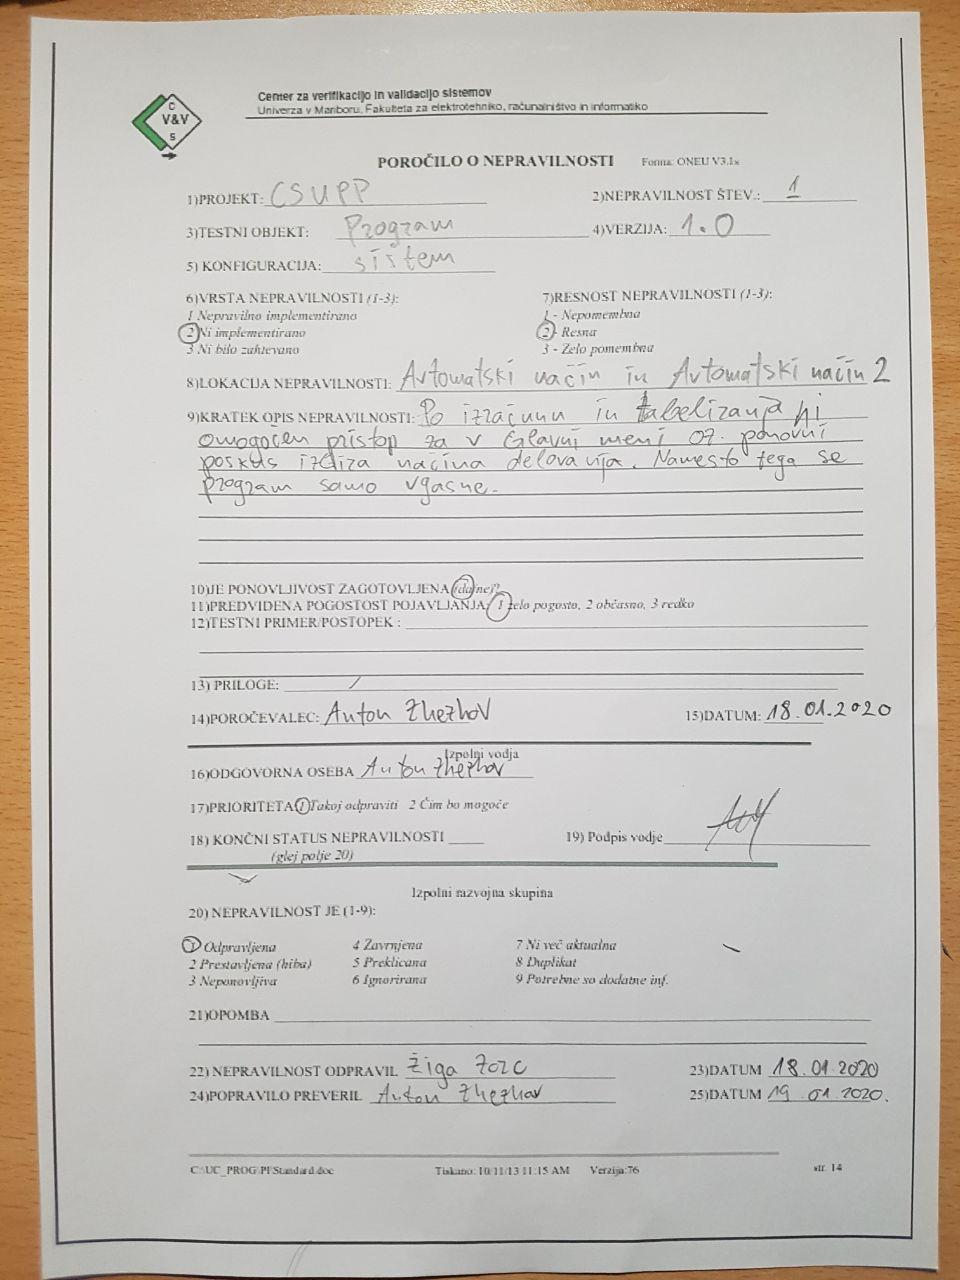
\includegraphics[width=15cm]{porocila/01.jpg}

\newpage
	
	\hspace{2cm}

	\vspace{2cm}

	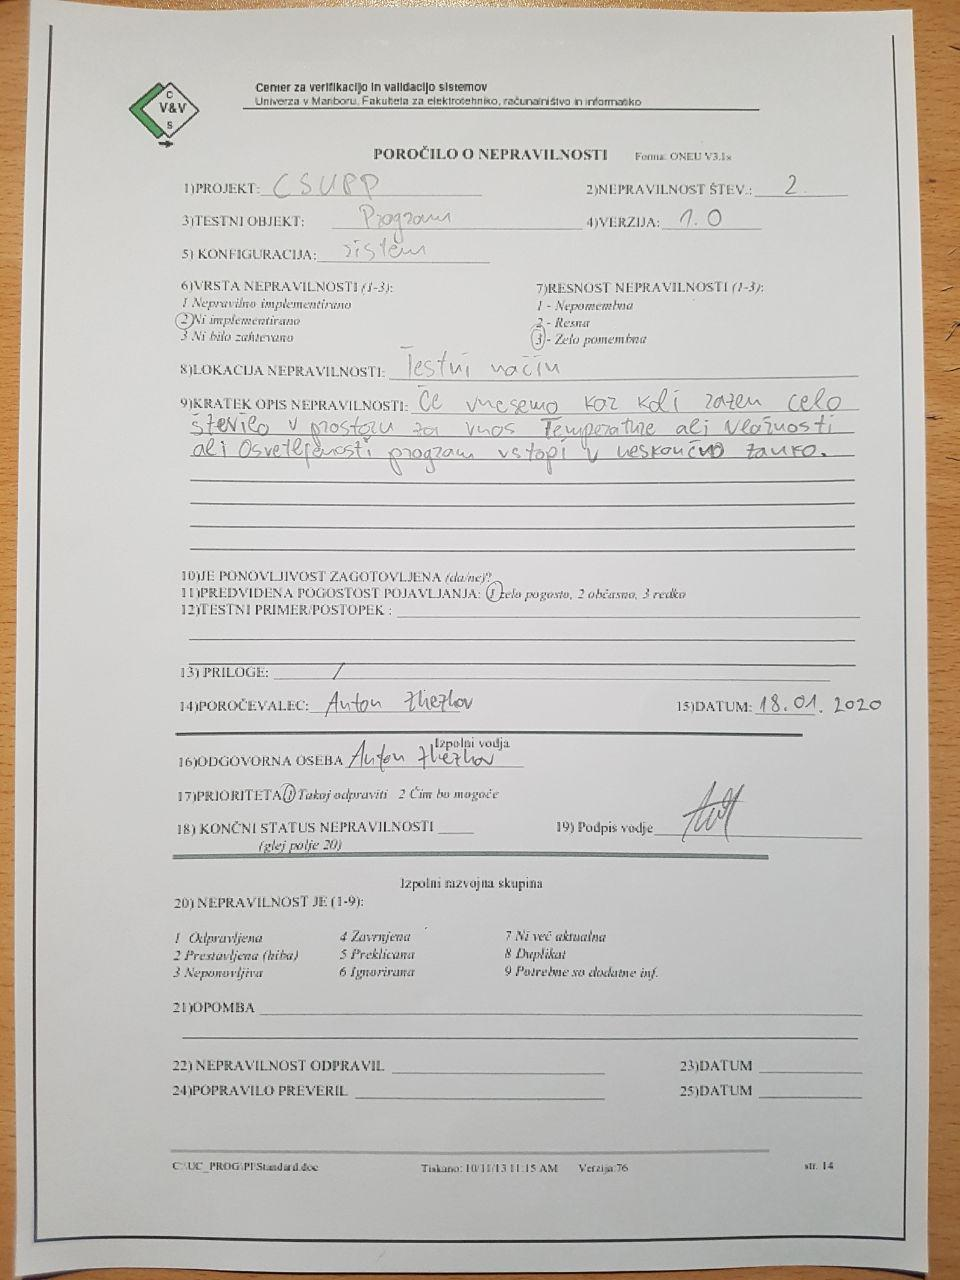
\includegraphics[width=15cm]{porocila/02.jpg}

\newpage

	\hspace{2cm}

	\vspace{2cm}
	
	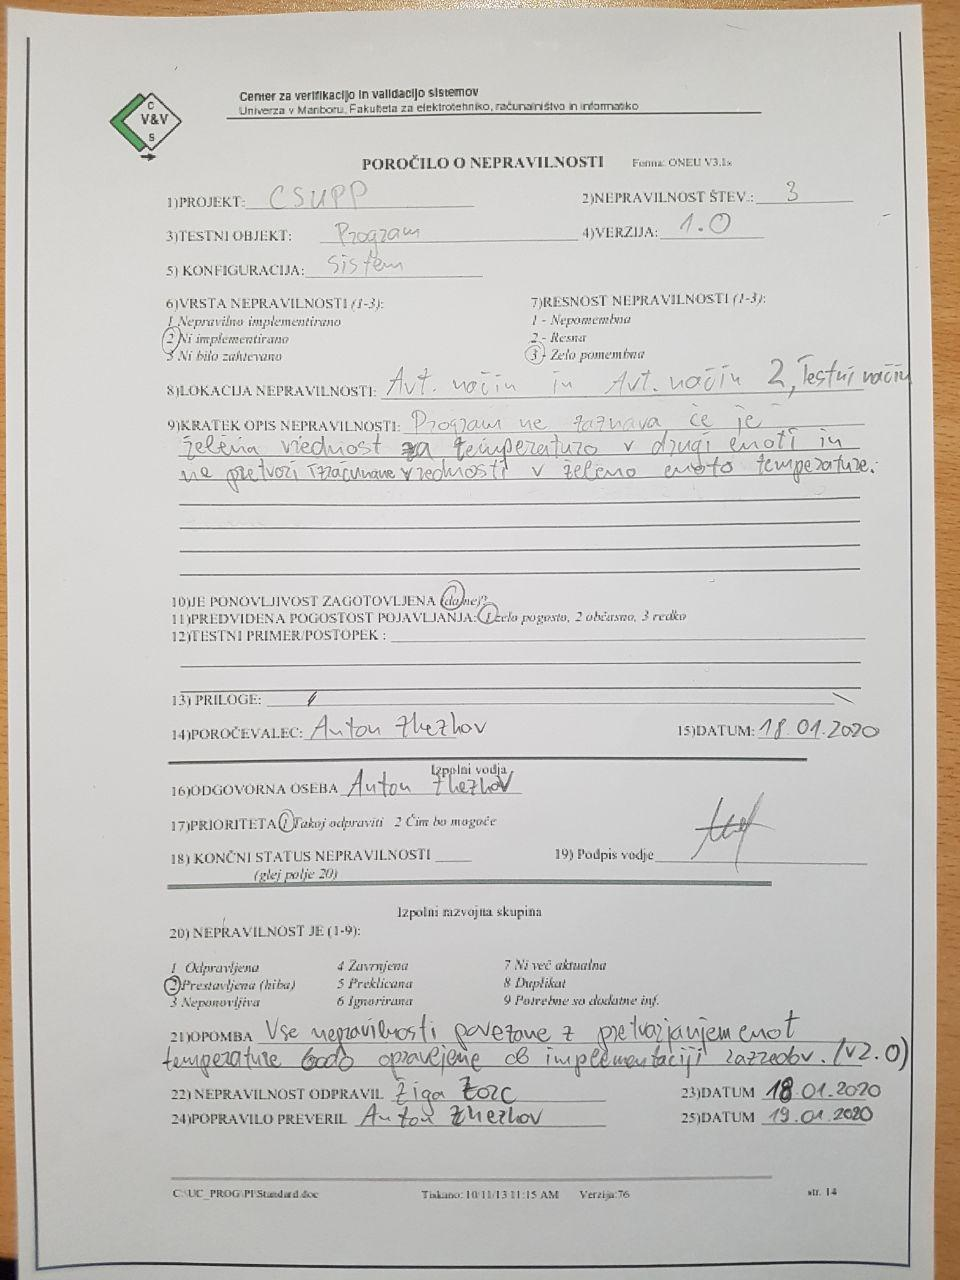
\includegraphics[width=15cm]{porocila/03.jpg}
	
\newpage
	
	\hspace{2cm}

	\vspace{2cm}
	
	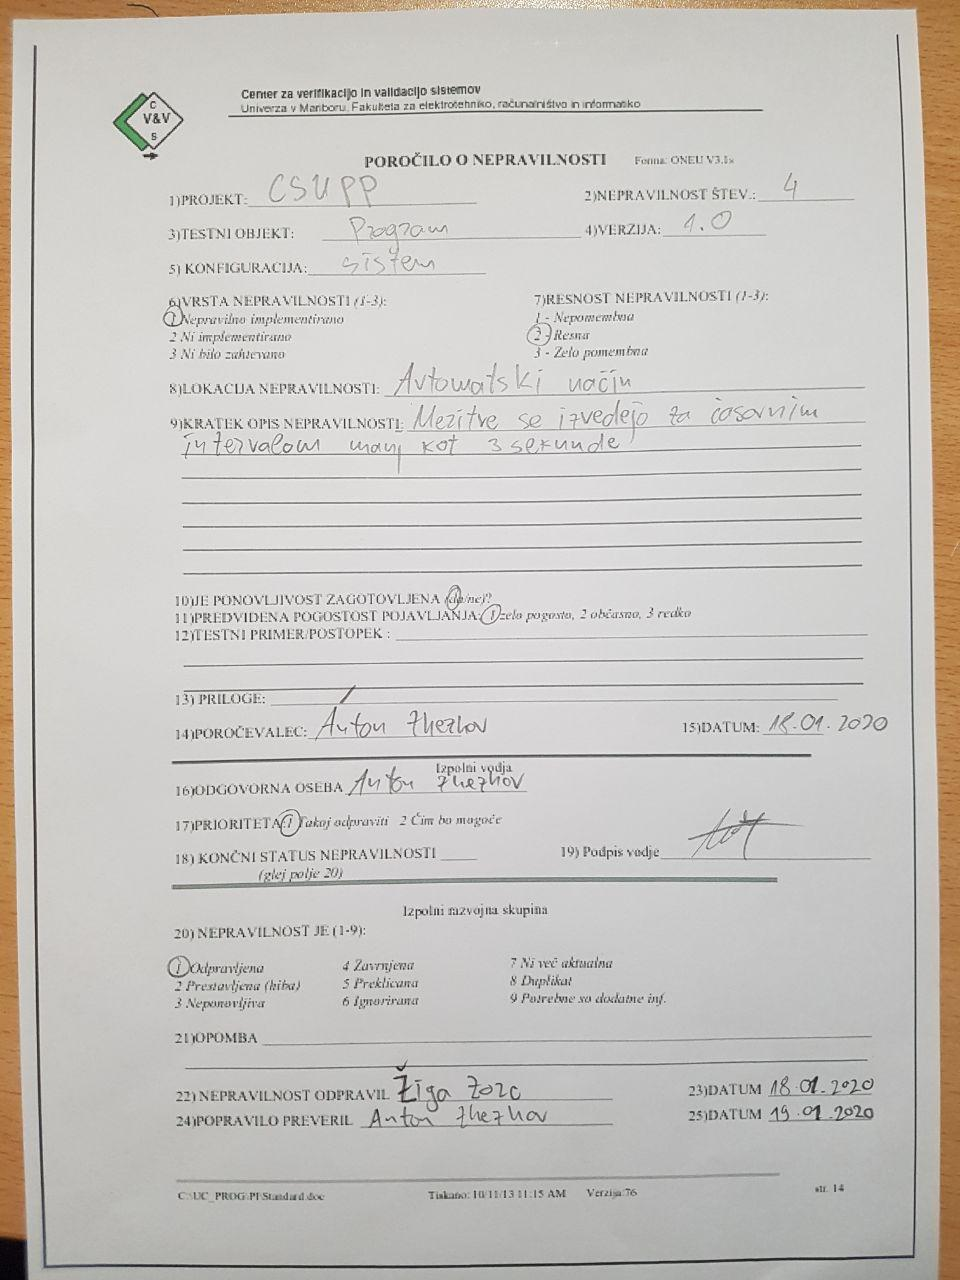
\includegraphics[width=15cm]{porocila/04.jpg}
	
\newpage
	
	\hspace{2cm}

	\vspace{2cm}
	
	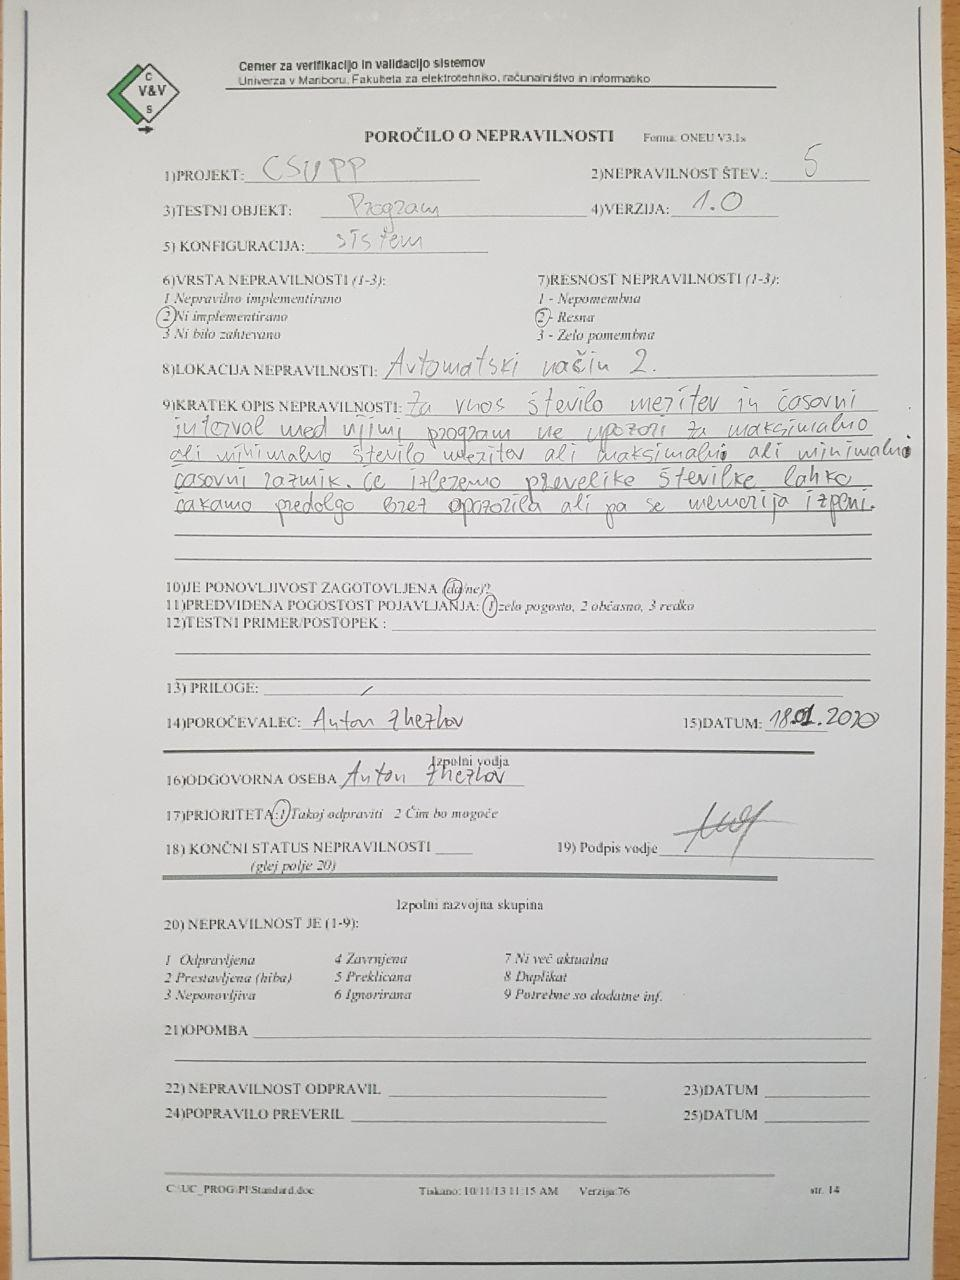
\includegraphics[width=15cm]{porocila/05.jpg}
	
\newpage
	
	\hspace{2cm}

	\vspace{2cm}
	
	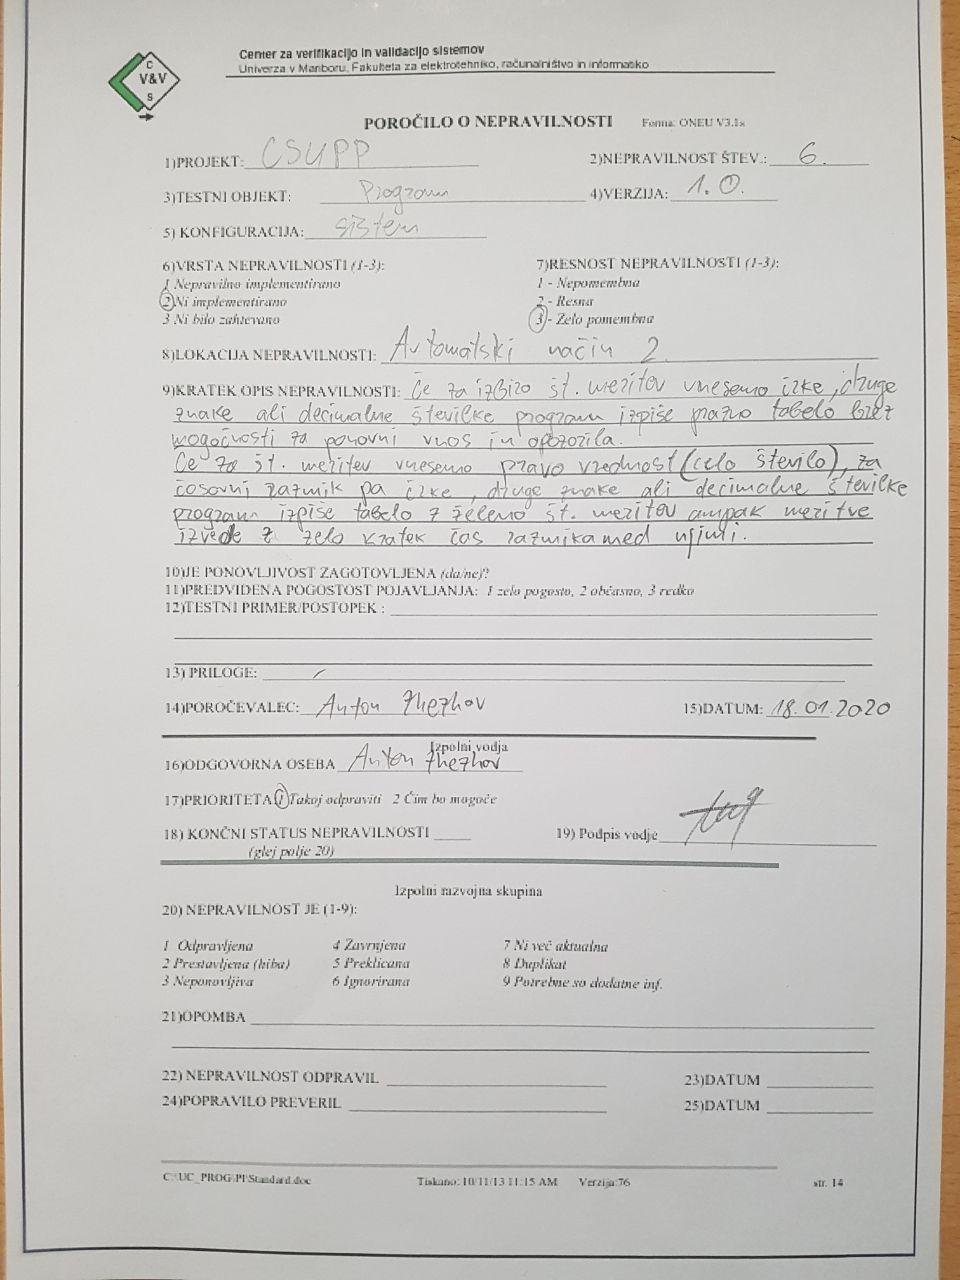
\includegraphics[width=15cm]{porocila/06.jpg}
	
\newpage
	
	\hspace{2cm}

	\vspace{2cm}
	
	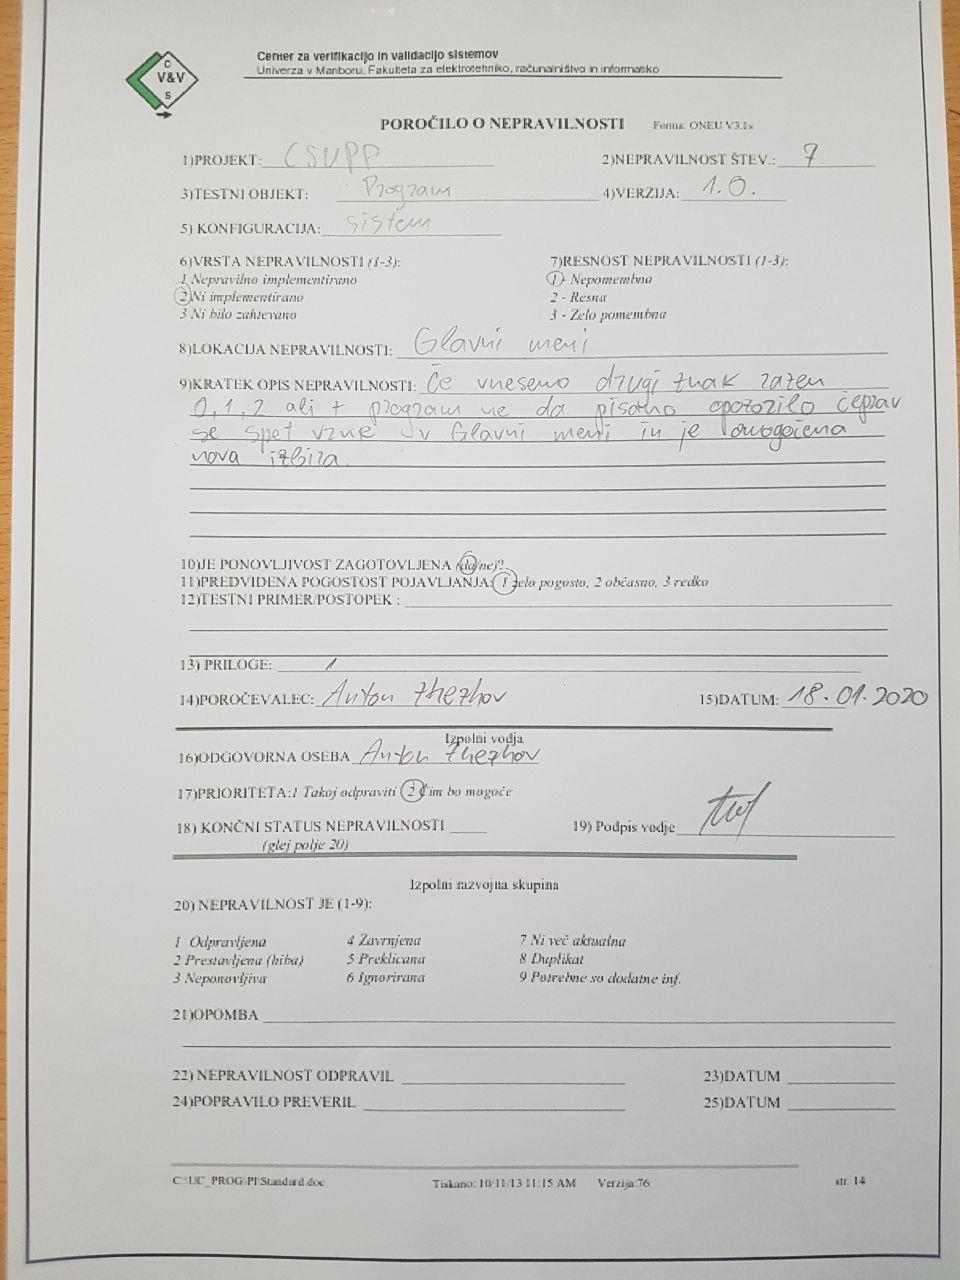
\includegraphics[width=15cm]{porocila/07.jpg}
	
\newpage
	
	\hspace{2cm}

	\vspace{2cm}
	
	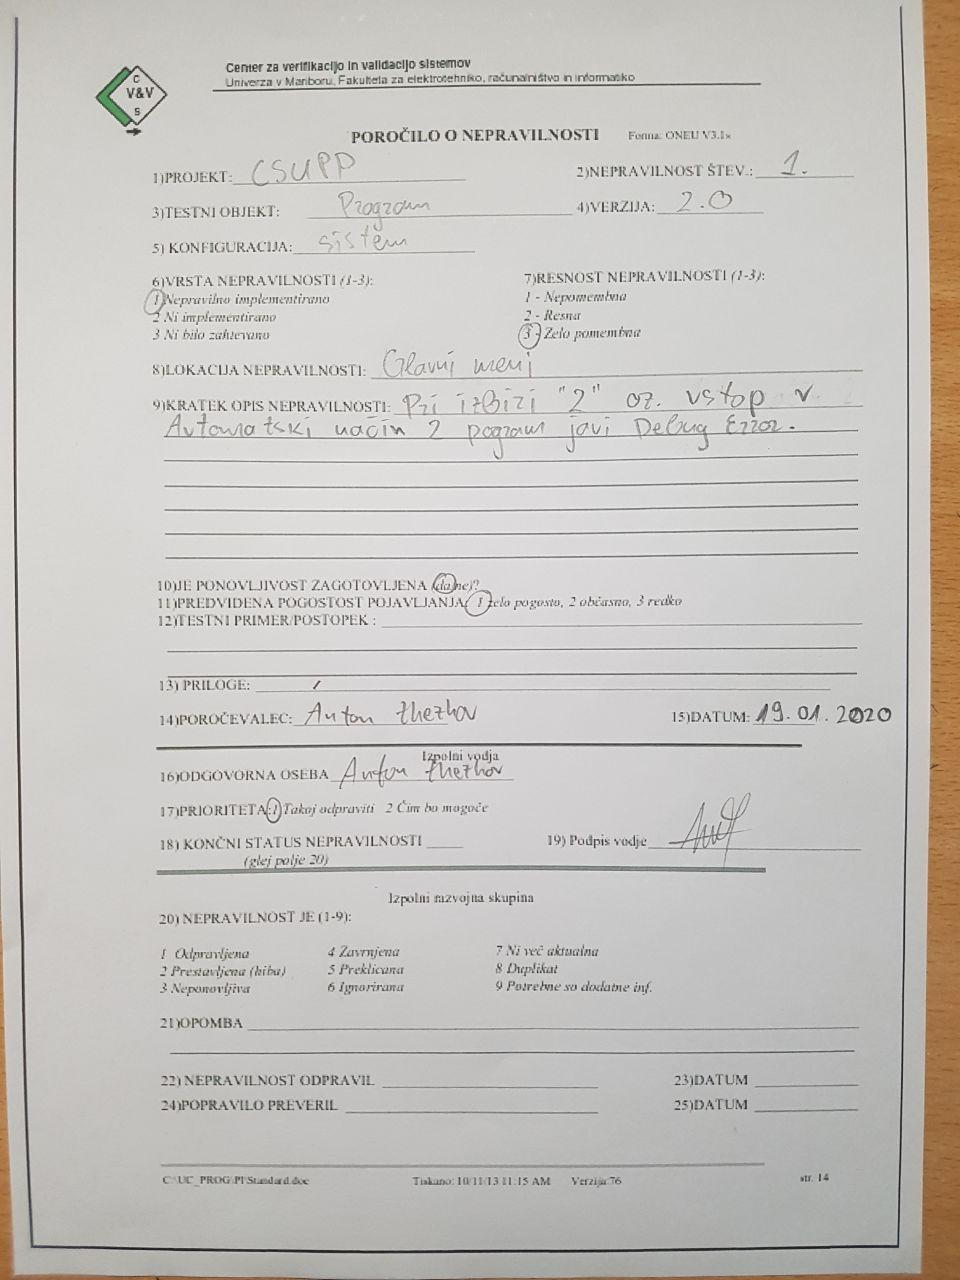
\includegraphics[width=15cm]{porocila/08.jpg}
	
\newpage
	
	\hspace{2cm}

	\vspace{2cm}
	
	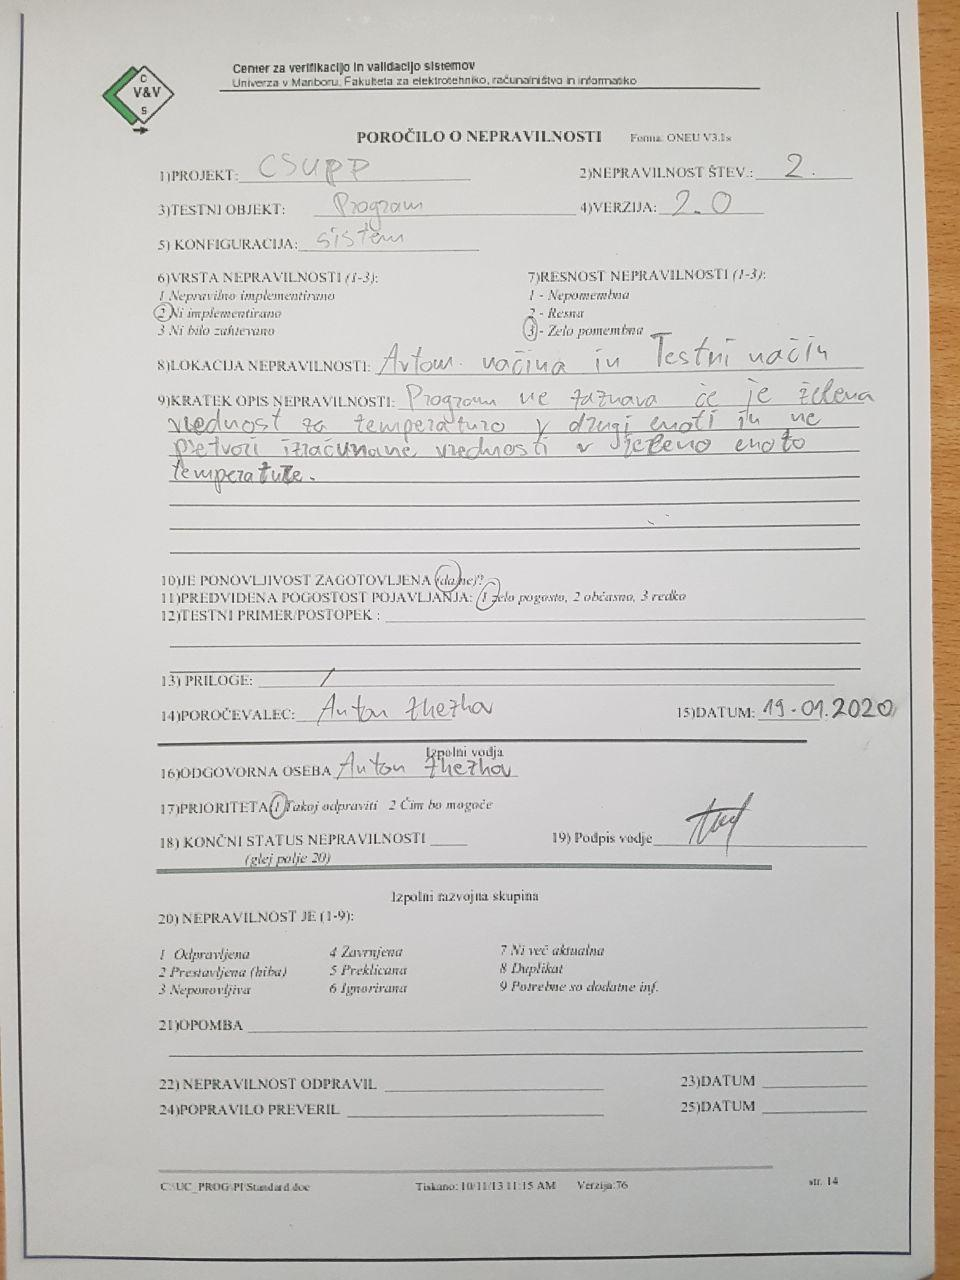
\includegraphics[width=15cm]{porocila/09.jpg}
	
\newpage
	
	\hspace{2cm}

	\vspace{2cm}
	
	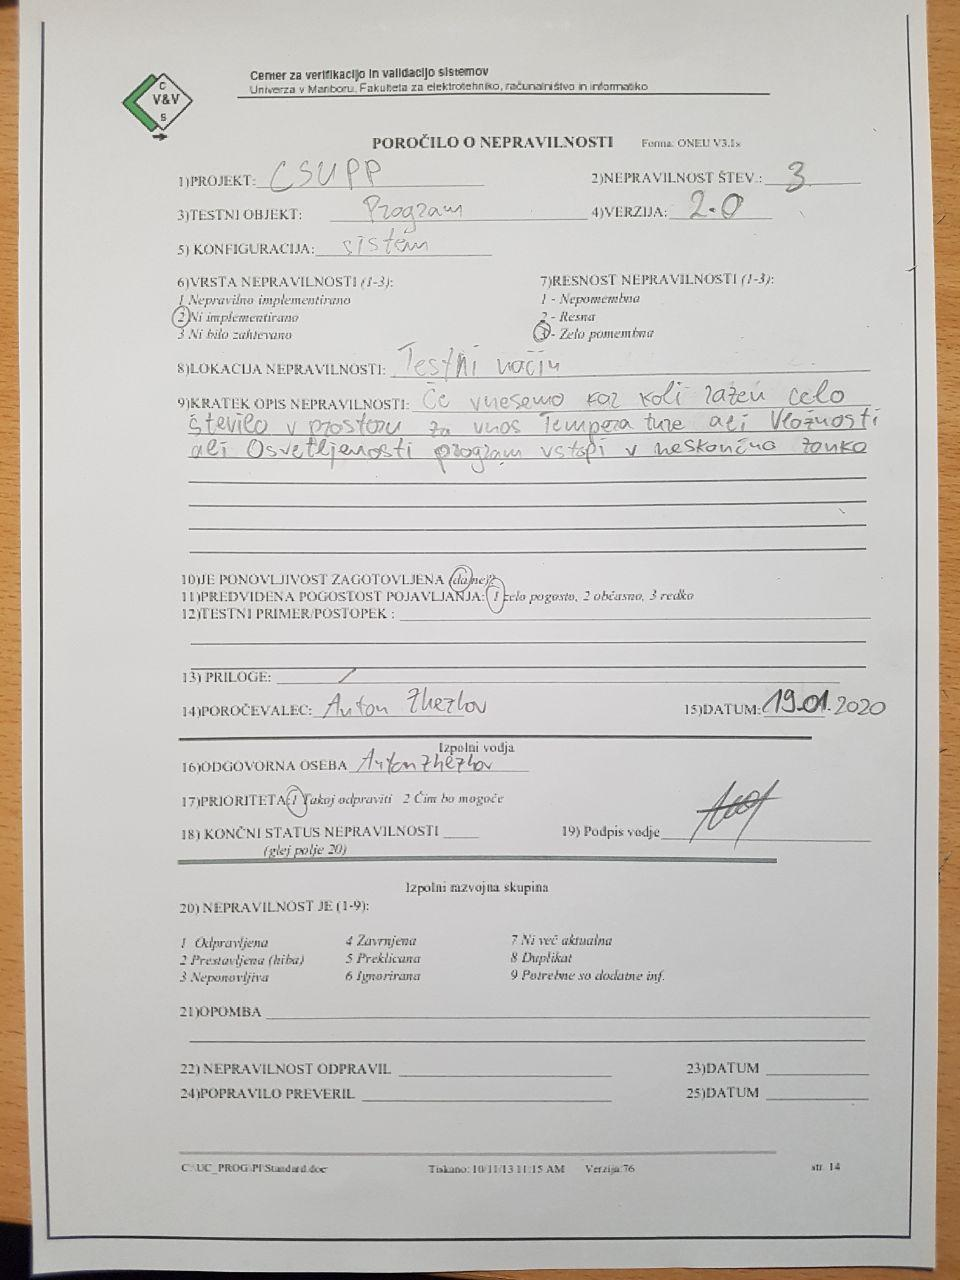
\includegraphics[width=15cm]{porocila/10.jpg}

}

\newpage

	\subsection{Podatki o kompleksnosti}

	\qquad Dobim napako pri uporabi programa CCCC na Windows 10 in v Linux.

	\vspace{2cm}

	{

	\centering

	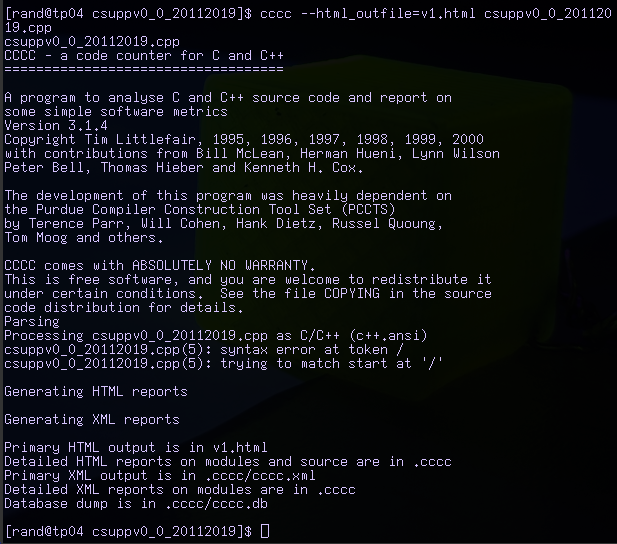
\includegraphics[width=14cm]{diagrami_slike/napaka_cccc.png}

	}


%\begin{comment}

\newpage

	\section{Načrtovalska dokumentacija}

		\subsection{Povzetek iz specifikacij}

			\subsubsection{Kontekstni nivo}

			{

			\centering

			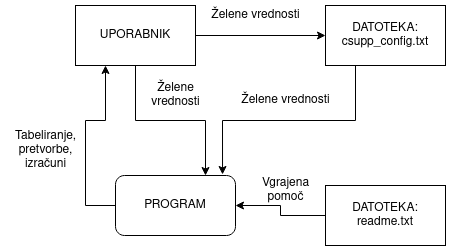
\includegraphics[width=8.5cm]{diagrami_slike/kont_nivo.png}

			}

			\subsubsection{Datoteke ki ih uporablja uporabnik}

			\qquad Uporabnik za delovanje programa potrebuje naslednje datoteke:

			\begin{itemize}

				\item csuppvX\_Y\_DD\_MM\_YYYY.exe (izvršljiva verzija programa)

				\item csupp\_config.txt (datoteka ki vsebuje ambientalne lasnosti in jo uporabnik spreminja po potrebi)

				\item readme.txt (besedilo vgrajene pomoči)

			\end{itemize}

			\subsubsection{Zagon programa}

			\qquad Program  zaženemo iz CMD tako da se moramo nahajati v datoteki programa, vtipkamo ime programama: 
			csuppvX\_Y\_DD\_MM\_YYYY.exe in pritisnemo Enter. Zaženemo  ga  lahko  tudi  iz  okenskega raziskovalca 
			z dvoklikom na njegovo ikono ali bližnjico. 

			\subsubsection{Datoteke ki jih potrebuje vzdrževalec}

			\begin{itemize}

				\item prijektna dokumentacija plan.pdf 
				\item csuppvX\_Y\_DD\_MM\_YYYY.cpp 
				\item functions.cpp
				\item functions.h
				\item csupp\_config.txt
				\item readme.txt

			\end{itemize}


		\subsection{Strukturni diagram}

		\qquad Kot tester bi potreboval konsultacije z razvajalcem za to točko.

		\subsection{Seznam modulov in podatkovnih tokov}
		
		\qquad Kot tester bi potreboval konsultacije z razvajalcem za to točko.
		
		\subsection{Opsi posameznih modulov}
		
		\qquad Kot tester bi potreboval konsultacije z razvajalcem za to točko.

		\subsection{Najpomembnejši parametri in opisi podatkovnih struktur}
			
			\subsubsection{Struktura datoteke csupp\_config.txt}

			\quad V tej datoteki uporabni ne-interaktivno vnese želene vrednosti za parametre.
			Datoteka vsebuje 6 vrstic, v vsako vrstico je napisano keri parameter ta vrstica predstavlja 
			in po dvopičju se zapišejo želene vrednosti. Primer formata:

			\quad PARAMETER: ŠTEVILO

			\quad TEMPERATURA: 25
			
			\quad PARAMETER: [ŠTEVILO, ŠTEVILO]
			
			\quad INTERVAL OSVETLJENOSTI: [4000, 7600]

			\subsubsection{Struktura datoteke readme.txt}

			\quad Datoteka vsebuje opis ukazov ki se izvajajo v procesu izračunov oz. tabeliranja. Format:

			\quad Oznaka ukaza - Opis oznake ukaza.

			\quad T2 - Izklopi grelec

			\quad V1 - Vklopi vlazilec

			\quad 03 - Izklopi luci

			\subsubsection{Parametri pri zagonu programa}

			\quad Ob  zagonu  pozna  program  en  sam  vhodni  parameter.  To  je  '-t'  (brez  narekovajev).  
			Služi  vklopu  testnega režima delovanja. Ko program poženemo s tem parametrom, ostane v testnem 
			režimu delovanja do naslednjega zagona.

		\subsection{Natančna identifikacija uporabljenih orodij in knjižnic}

			\begin{itemize}

				\item Za pisanje in prevajanje kode je bil uporabljan program 'Microsoft Visual Studio 2019'.
				\item Za pisanje dokuemntacije je bil uporaben pogram 'vim' za pisanje in urejanje tekstovne datoteke.
				\item Za pretvorbo tekstovne datoteke v PDF formatu je bil uporabljen program 'vim-live-latex-preview'.
				\item Za izdelavo csuppv\_config.txt in readme.txt  datotek je bil uporabljen standardni program 'Microsoft Notepad'.

			\end{itemize}

		\subsection{Postopek potreben za ustvarjanje izvršilne kode}

			\qquad Kot tester bi potreboval konsultacije z razvajalcem za to točko.

%\end{comment}

\newpage

	{
	\centering

	\hspace{0cm}

	\vspace{4cm}

	{\large{Program}}

	\vspace{1cm}

	{\bf{\Huge{Centralni sistem za upravljanje poslovnega prostora}}}

	\vspace{0.5cm}

	{(verzija 2.0)}
	
	\vspace{1.5cm}

	{\bf{\Large{Uporabniški priročnik}}}

	{
	\color{white} \section{Blank white}
	}
	}

\newpage

	\subsection{Namen}

	\quad Program je izdelan kot simulator in ima za namen krmiljenje temperature, vlage in osvetljenosti v prostoru.

	\subsection{Strojne in programske zahteve}

	\quad Program dela v okolju Windows, nima gafičnega vmesnika, deluje kot konzolna aplikacija oz. lahko deluje
	tudi na starejše računalnike z starejšo verzijo okolja Windows.

	\subsection{Namestitev in zagon programa}

	\quad Program je v mapo z dvema datotekama (csupp\_config.txt in readme.txt) ki sta pomembni za delovanje programa.
	V datoteko csupp\_config.txt so že nastavljeni parametri kot primer, uporabnik ih lahko spreminja po svojo željo.
	
	\hspace{-0.8cm} \quad Program zaženemo z dvoklikom na ikono programa csuppvX\_Y\_DD\_MM\_YYYY.exe ali pa preko CMD okolja se predstavimo
	v mapo v kero se nahaja program in ga zaženemo z komando: \\ ./csuppvX\_Y\_DD\_MM\_YYYY.exe .

	\hspace{-0.8cm} \quad Preko okolja CMD lahko tudi zaženemo program z argumentom '-t':\\ ./csuppvX\_Y\_DD\_MM\_YYYY.exe -t .
	Tako pridemo v testnem načinu delovanja programa ki je namenjen testerju ali razvijalcu za preizkus programa, ne pa uporabniku.

	\subsection{Navodilo za uporabo}

	\subsubsection{Glavni meni}

	\quad Ko program zaženemo se prikaže Glavni meni ki ponuja 4 izbire: Izhod, Avtomatski način, Avtomatski način 2 in Pomoč. Želeno funkcijo 
	programa izberemo tako da vpišemo številko ali znak pred funkcijo ki jo želimo.

	\subsubsection{Izhod}

	\quad Če želimo izhod iz programa vtipkamo '0' (nulo) in pritisnemo Enter in se program zapre.

	\subsubsection{Avtomatski način}

	\quad Za izbiro tega načina vtipkamo 1 (ena) in pritisnemo Enter, program si sam izmisli in izpiše izmisljene vrednosti in začne
	izvajati izračune, tabeliranje in ukaze za regulacijo na vsake 3 sekunde za 100 meritve. Na koncu izračunov izpiše še
	povrpečne vrednosti parametrov in odstopanje.

	\subsubsection{Avtomatski način 2}

	\quad Ta način izberemo če vtipkamo 2 (dve) in pritisnemo Enter, dobimo mogočnost za dva vnosa in sicer število meritev in
	razmik med njimi. Vnesemo število meritev kot celo števolo in pritisnemo Enter, vnesemo še želen čas kot celo število v milisekundah
	in pritisnemo Enter. Program začne izvajati izračune, tabeliranje in ukaze za regulacijo in na koncu izpiše povprečne vrednosti in 
	odstopanja glede naše zelene vrednosti v datoteki.
	
	\subsubsection{Pomoč}

	\quad Če izberemo znak + se izpiše pomoč za uporabo programa in opis ukazov ki se izvajajo. Lahko poiščemo pomoč vsakič ko
	nam je ponujen interaktivni vnos v programu oz. v vsakem načinu delovanja programa.
\end{document}
